\newcommand{\Kernel}[1]{\ensuremath{w_{\sigma}(#1)}}

\paragraph{Saliency-aware normal estimator.}
We propose a new normal estimator on digital surfaces, which uses
the visibility of the point of interest while taking into account
a user-given scale $\sigma$. If $\sigma$ is proportionnal to the
average length between visible points (so some
$\Theta\left(\sqrt{h}\right)$), then this estimator is observed to be
multigrid convergent along digitization of smooth shapes. However,
since the computation window is limited by the visibility, it
better approximates the geometry near sharp or salient features.

More precisely, we choose a Gaussian function
$\Kernel{x}\coloneqq e^{-\frac{x^2}{2\sigma^2}}$ as a weight kernel. Let
$V_p$ be the set of visible points from the point $p$. Let $c_p$
be the weighted centroid of the visible points around $p$,
i.e. $c_p \coloneqq \frac{\sum_{q \in V_p} \Kernel{\|q-p\|}q}{\sum_{q \in
V_p} \Kernel{\|q-p\|}}$. We form the weighted covariance matrix
$\mathcal{V}_p$ of the points $V_p$ as:
\begin{equation}
    \mathcal{V}_p = \sum_{q \in V_p} \Kernel{\|q-p\|}(q - c_p)(q - c_p)^T.
\end{equation}
The \emph{visibility normal} $\vec{n}(p)$ of point $p$ at scale $\sigma$ is defined
as the first eigenvector of the covariance matrix $\mathcal{V}_p$
of the visible points, corresponding to its smallest
eigenvalue. Its orientation is chosen to point in the same
direction as the average of the trivial normals to the surfels
touching the point $p$.


\paragraph{Experimental validation.} [TO COMPLETE]
Figure~\ref{fig:normals-estimation} shows an example
of our normals compared to normals computed with the integral invariant (II) estimator~\cite{Lachaud:2017-lnm}.

\begin{figure}
    \centering
    \begin{tabular}{c c}
        \begin{tikzpicture}
            \centering
            \begin{axis}[
                width=0.53\textwidth,
                xlabel={Gridstep},
                ylabel={RMSE error},
                x dir=reverse,
                legend pos=north east,
                ymajorgrids=true,
                grid style=dashed,
                ymode=log,
                xmode=log,
                log ticks with fixed point,
            ]
                \addplot[
                    color=cyan,
                ] coordinates {
                    (0.125,0.0156736)(0.250,0.031503)(0.375,0.0384303)(0.500,0.0441086)(0.625,0.0418896)(0.750,0.0584604)(0.875,0.065503)(1.000,0.0729735)
                };
                \addplot[
                    color=red,
                ] coordinates {
                    (0.125,0.0221236)(0.250,0.0317159)(0.375,0.0542242)(0.500,0.0706101)(0.625,0.09481)(0.750,0.134544)(0.875,0.130578)(1.000,0.127371)
                };
                \addplot[
                    color=MyGreen,
                ] coordinates {
                    (0.125,0.0203851)(0.250,0.032289)(0.375,0.0353311)(0.500,0.0568694)(0.625,0.0665957)(0.750,0.106711)(0.875,0.0817172)(1.000,0.104688)
                };
                \addplot[
                    color=orange,
                ] coordinates {
                    (0.125,0.0106125)(0.250,0.0223176)(0.375,0.032738)(0.500,0.0365776)(0.625,0.0362568)(0.750,0.0181232)(0.875,0.0303189)(1.000,0.0263066)
                };
                \addplot[
                    color=black,
                    thick,
                    domain=0.1:1,
                    samples=200,
                ] {0.1*x^(0.5)};
            \end{axis}
        \end{tikzpicture} &
        \begin{tikzpicture}
            \centering
            \begin{axis}
                [
                width=0.53\textwidth,
                xlabel={Gridstep},
                ylabel={$E_{\max}$ error},
                x dir=reverse,
                legend pos=north east,
                ymajorgrids=true,
                grid style=dashed,
                ymode=log,
                xmode=log,
                log ticks with fixed point,
                ]
                \addplot[
                    color=cyan,
                ] coordinates {
                    (0.125,0.0586128)(0.250,0.0736204)(0.375,0.114564)(0.500,0.114592)(0.625,0.136021)(0.750,0.152418)(0.875,0.139939)(1.000,0.234379)
                };
                \addplot[
                    color=red,
                ] coordinates {
                    (0.125,0.0743185)(0.250,0.0810657)(0.375,0.113504)(0.500,0.145859)(0.625,0.256274)(0.750,0.266855)(0.875,0.259101)(1.000,0.274269)
                };
                \addplot[
                    color=MyGreen,
                ] coordinates {
                    (0.125,0.0670488)(0.250,0.0926269)(0.375,0.0973621)(0.500,0.137059)(0.625,0.155913)(0.750,0.290065)(0.875,0.164799)(1.000,0.317625)
                };
                \addplot[
                    color=orange,
                ] coordinates {
                    (0.125,0.0313599)(0.250,0.044124)(0.375,0.0643389)(0.500,0.0684951)(0.625,0.0853552)(0.750,0.0532733)(0.875,0.064386)(1.000,0.0873334)
                };
                \addplot[
                    color=black,
                    thick,
                    domain=0.1:1,
                    samples=200,
                ] {0.1*x^(0.5)};
            \end{axis}
        \end{tikzpicture} \\
        \multicolumn{2}{c}{
            \begin{tikzpicture}
                \begin{axis}[
                    hide axis,
                    xmin=0, xmax=1,
                    ymin=0, ymax=1,
                    legend columns=5,
                    legend style={
                        at={(0.5,-0.2)},
                        anchor=north,
                        draw=none,
                        column sep=15pt
                    }
                ]
            \addlegendimage{color=cyan}
            \addlegendentry{ellipsoid}
            \addlegendimage{color=red}
            \addlegendentry{goursat}
            \addlegendimage{color=MyGreen}
            \addlegendentry{rcube}
            \addlegendimage{color=orange}
            \addlegendentry{sphere9}

            \addlegendimage{color=black,thick};
            \addlegendentry{$0.1\sqrt{h}$}
                \end{axis}
            \end{tikzpicture}
        } \\
    \end{tabular}
    \caption{Error RMSE and $E_{\max}$ as a function of grid resolution}
    \label{fig:errors-normals}
\end{figure}

\begin{figure}
    \centering
    \begin{tabular}{|c||c|c|}
        \hline
        Normals & With cube edges & Flat (no shading) \\
        \hline
        \hline
        \raisebox{18mm}{II} &
        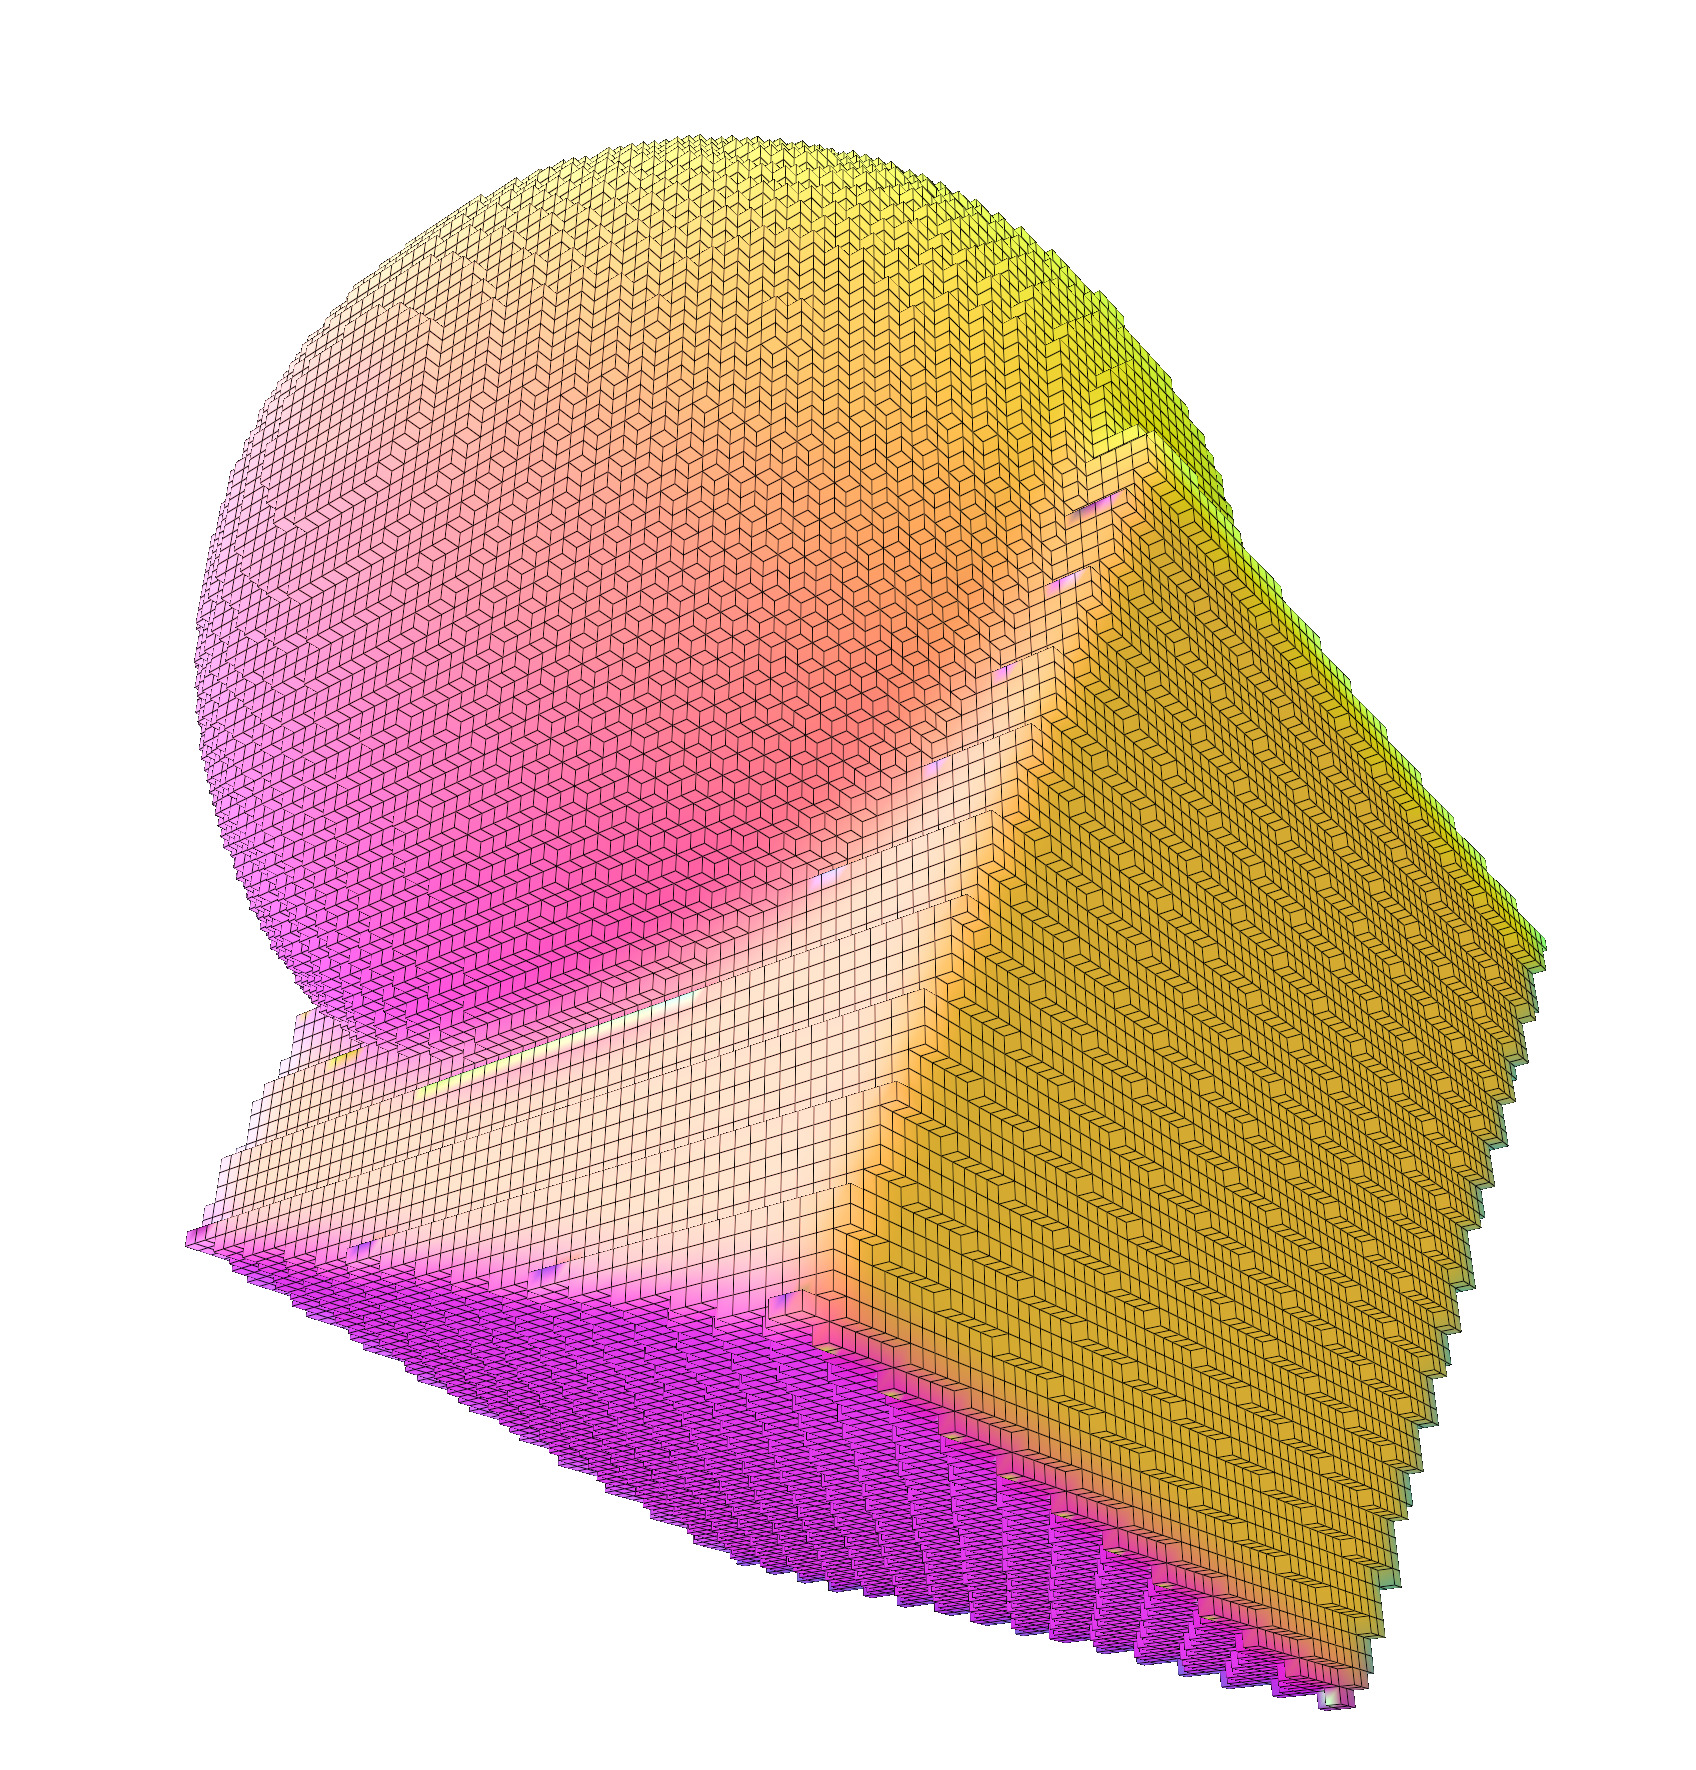
\includegraphics[width=0.3\textwidth]{pictures/cps-IIN-flat-edge} &
        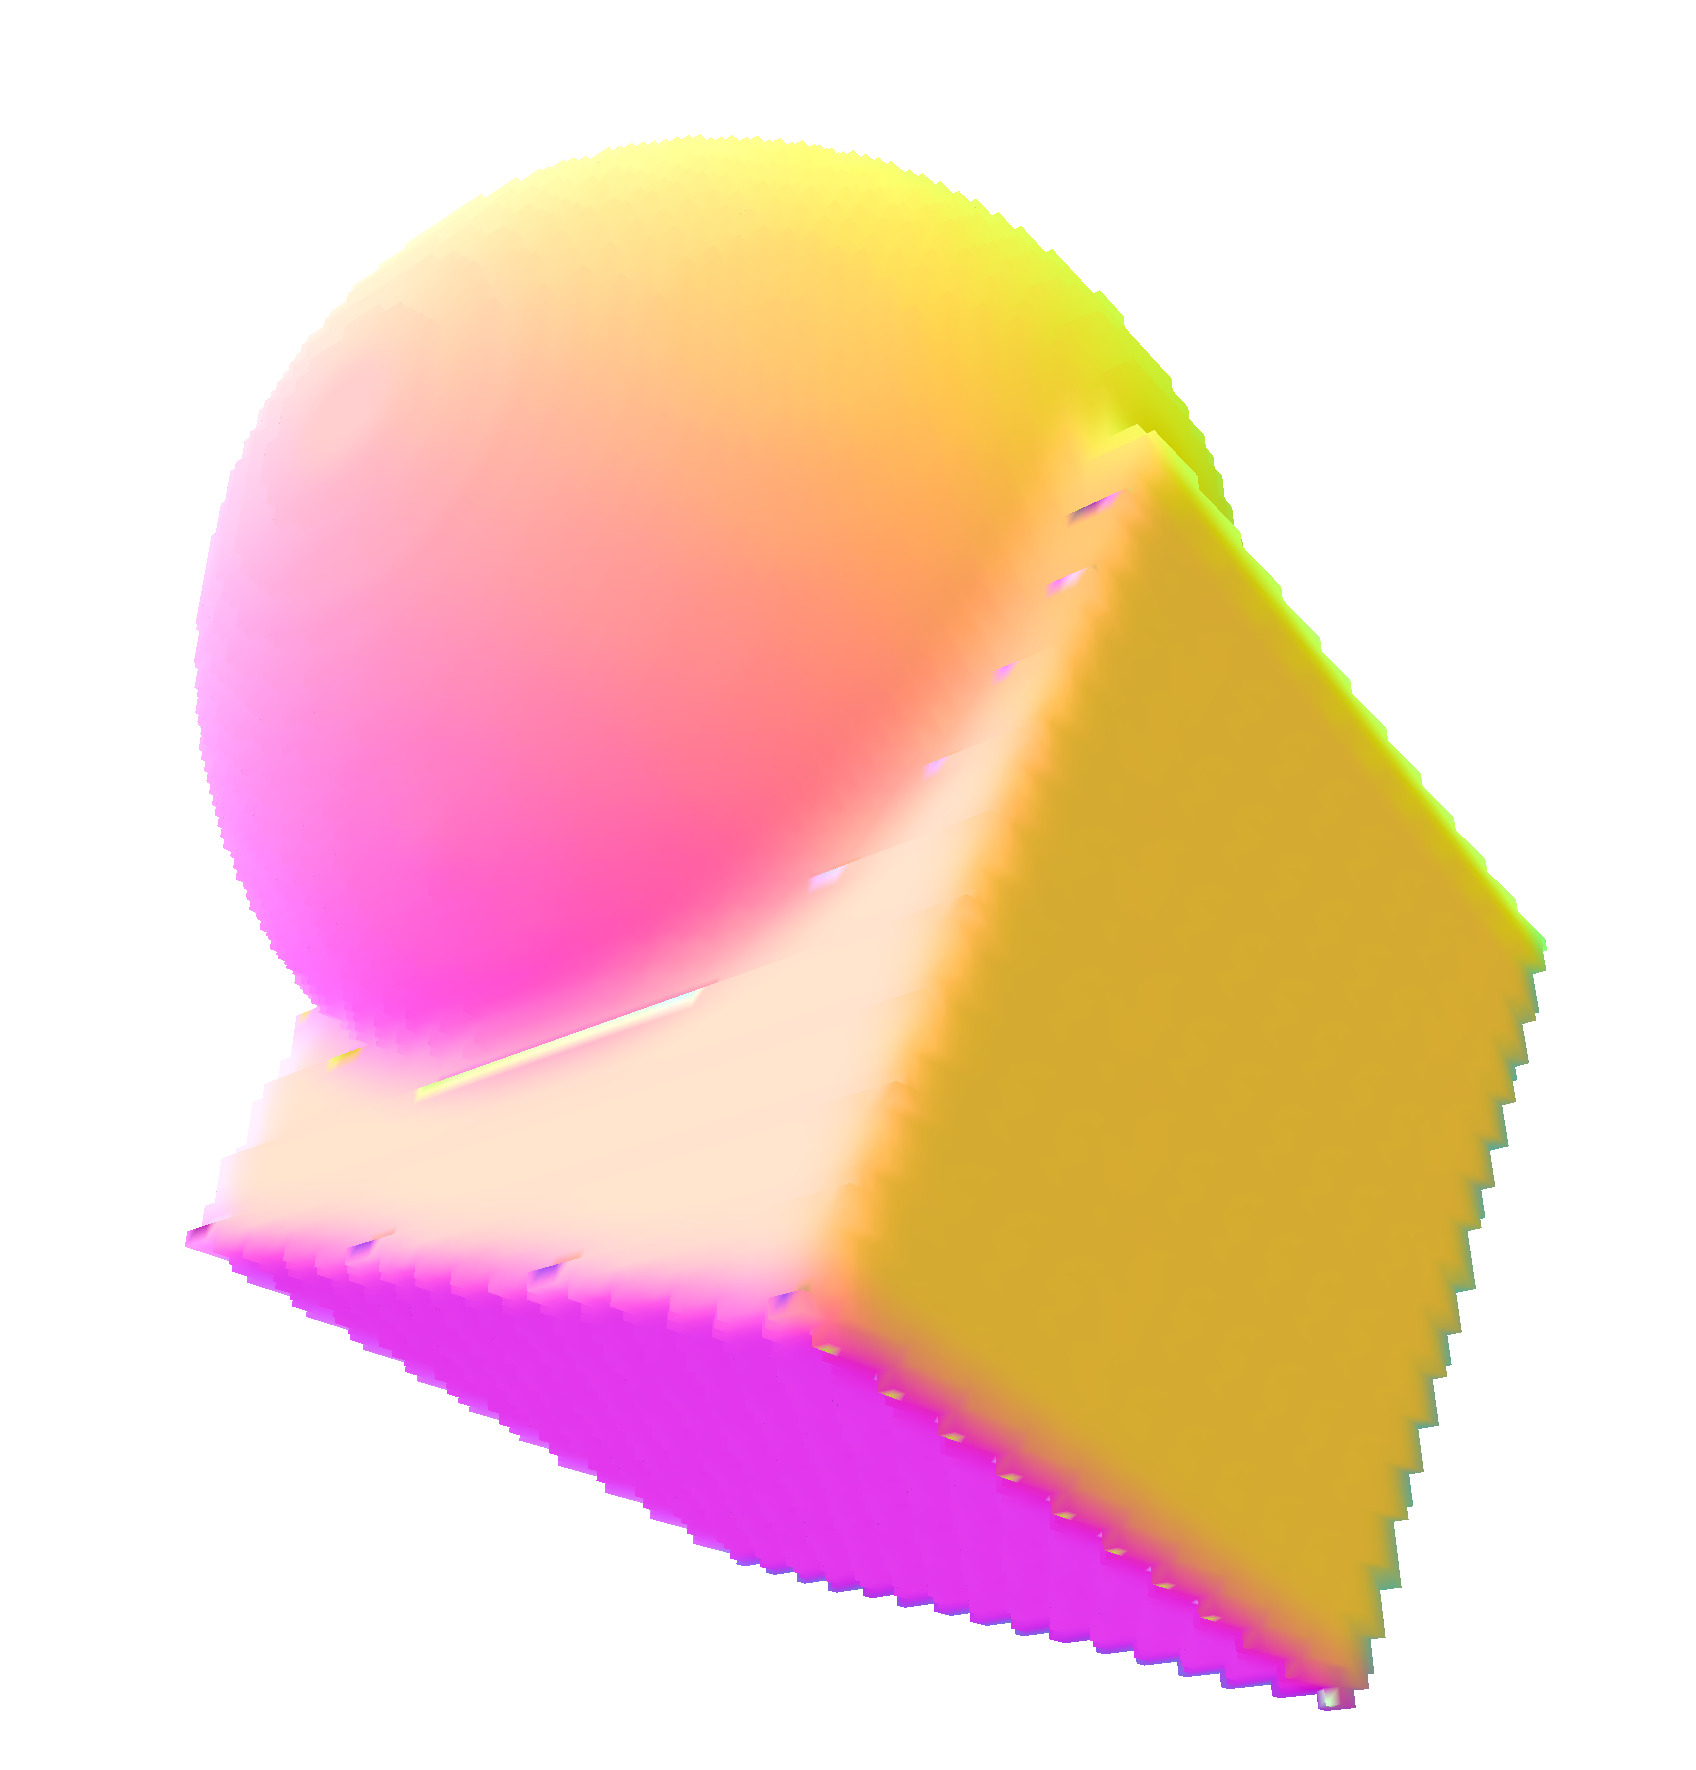
\includegraphics[width=0.3\textwidth]{pictures/cps-IIN-flat} \\
        %% 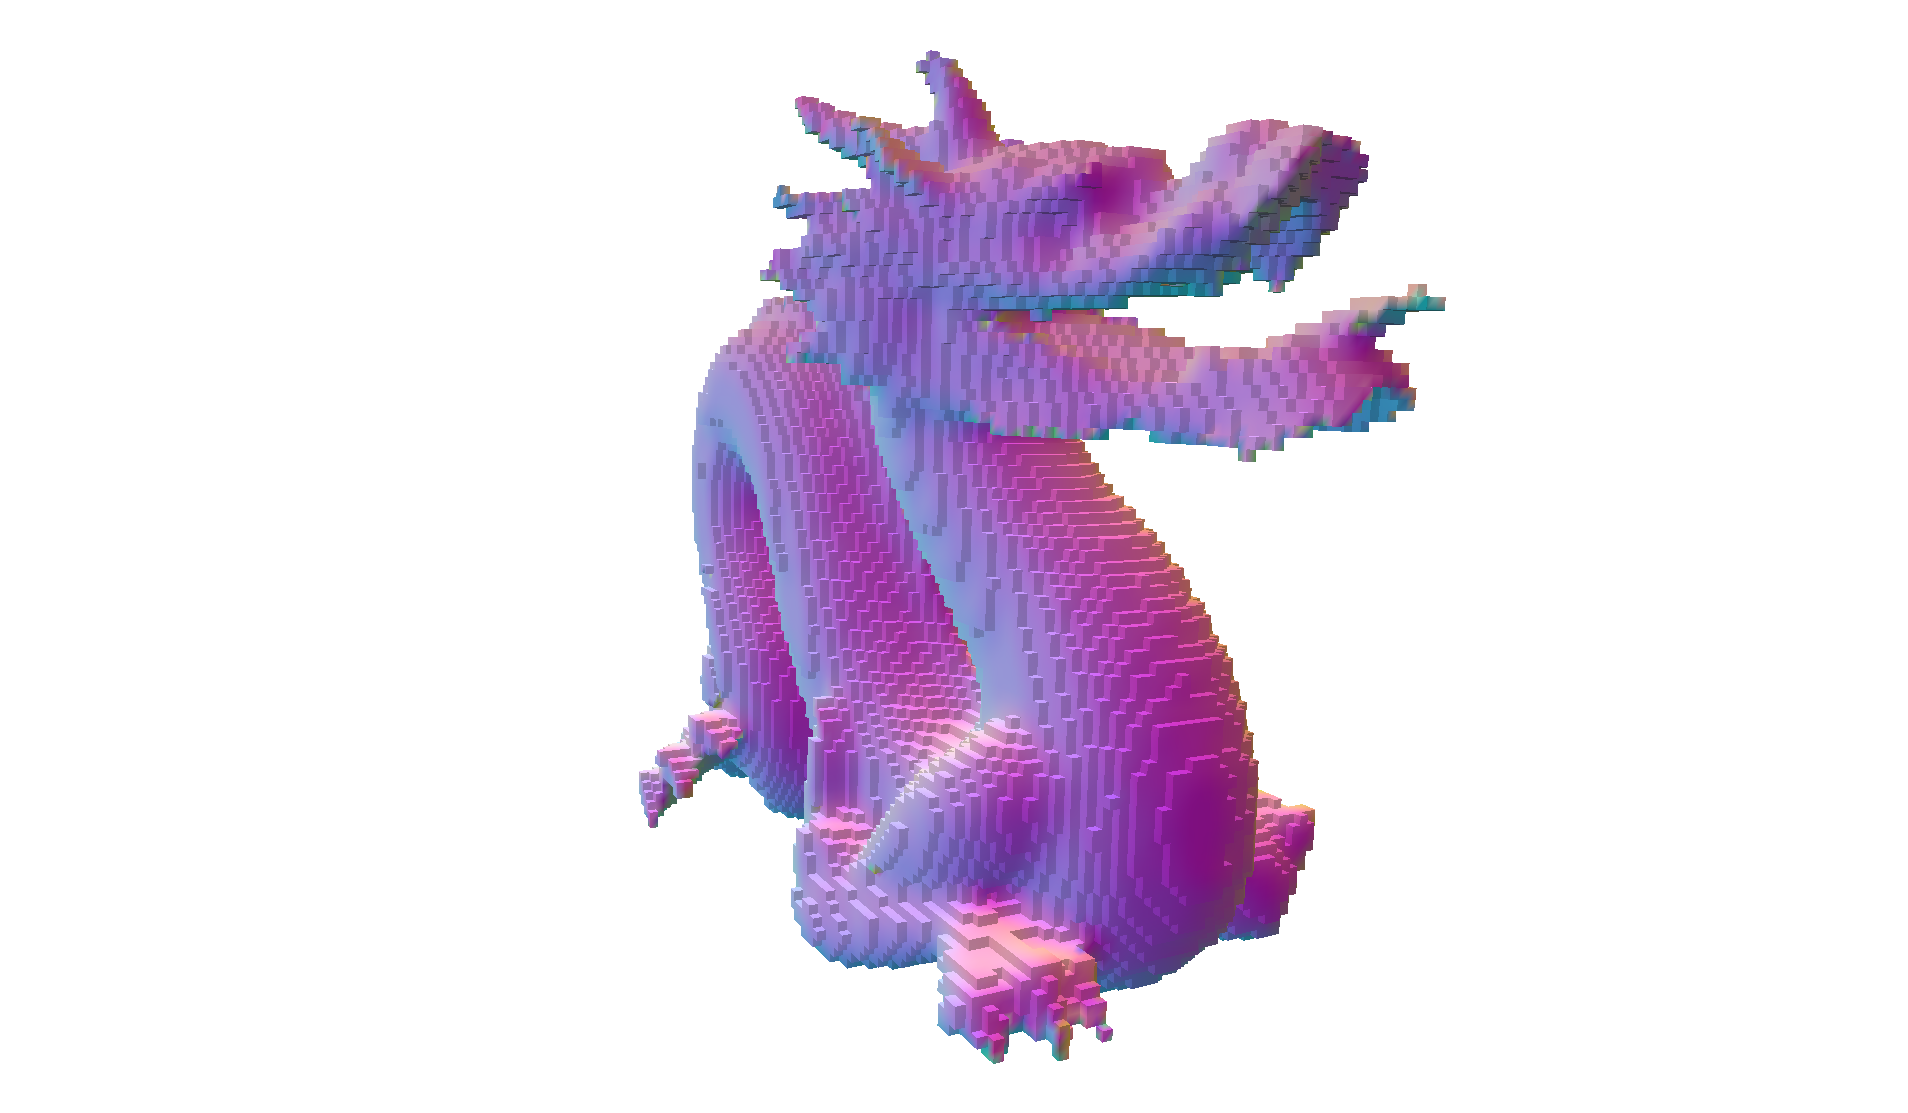
\includegraphics[width=0.4\textwidth]{pictures/chinese-dragon-normal-estimation-cubes-II} &
        %% 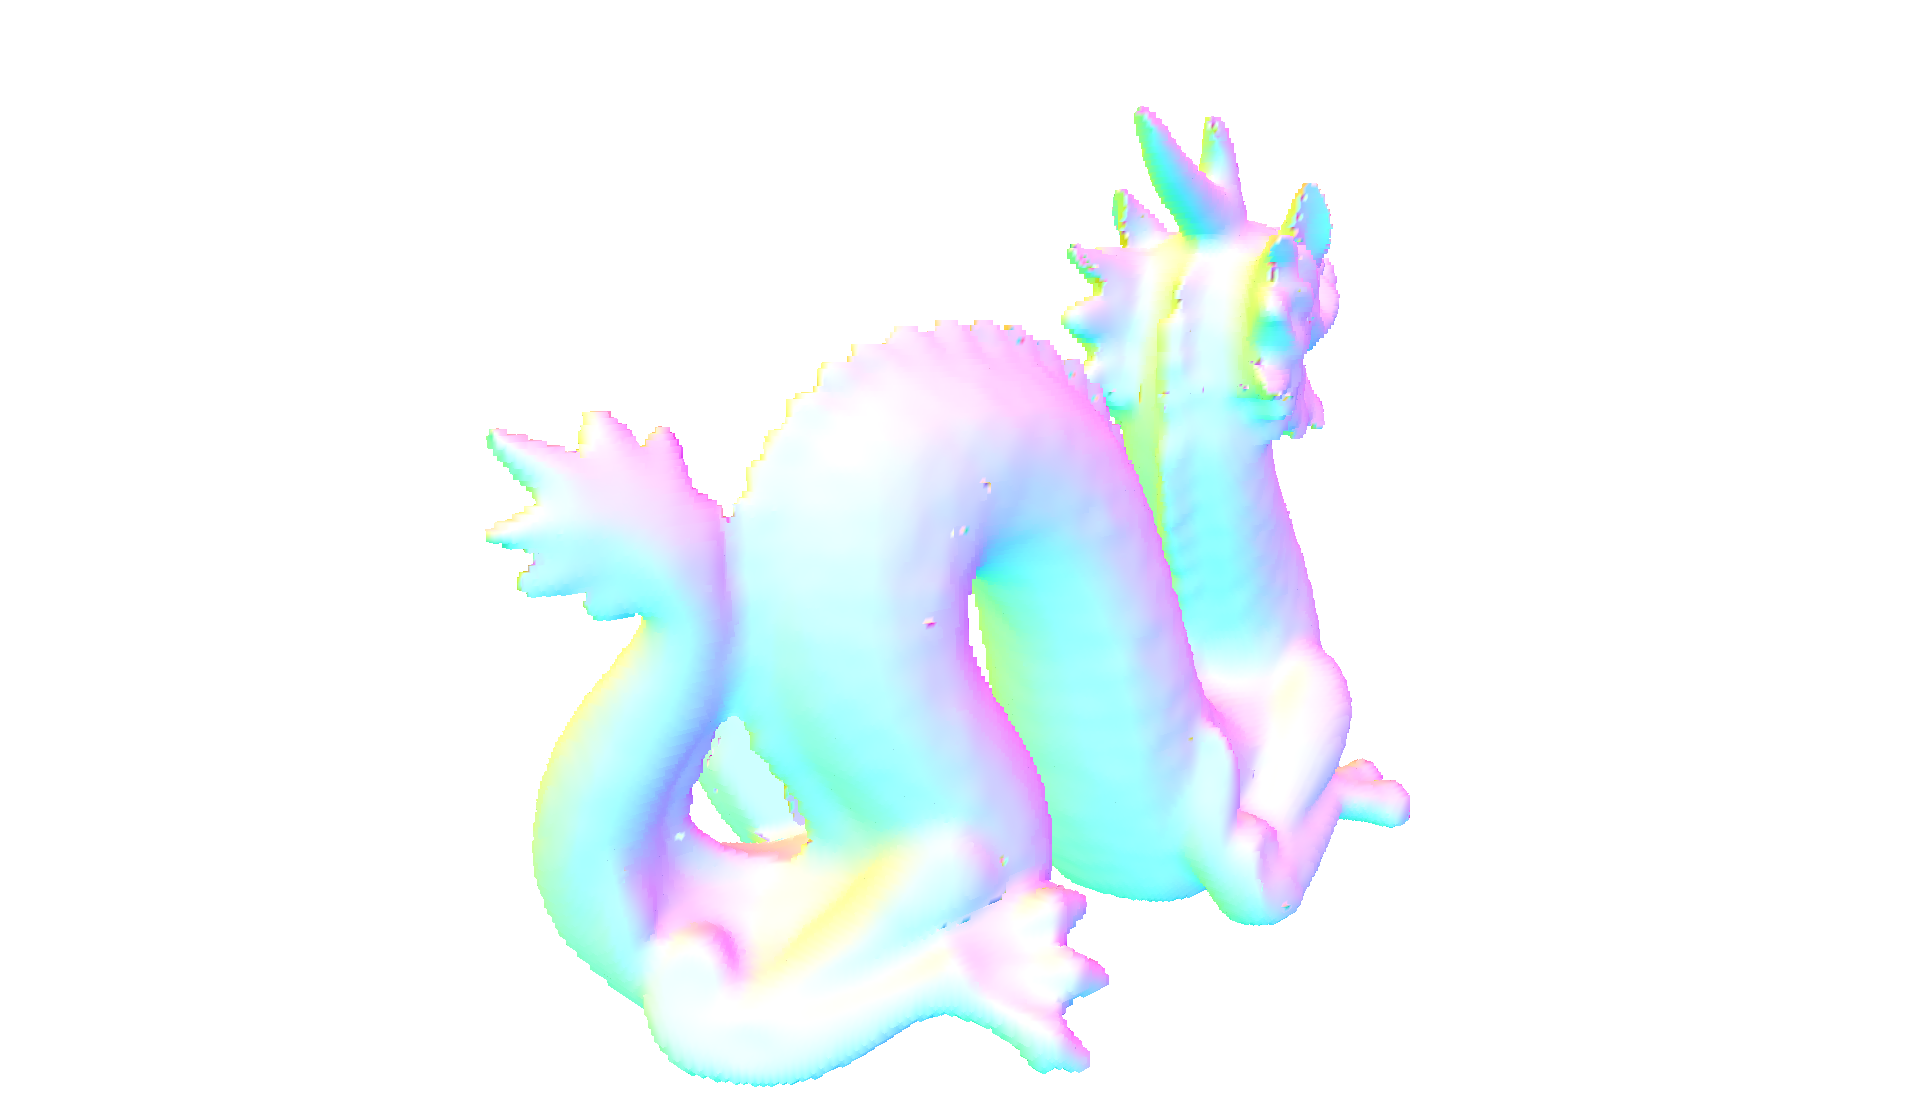
\includegraphics[width=0.4\textwidth]{pictures/chinese-dragon-normal-estimation-smooth-II} \\
        \hline
        \raisebox{18mm}{Ours} &
        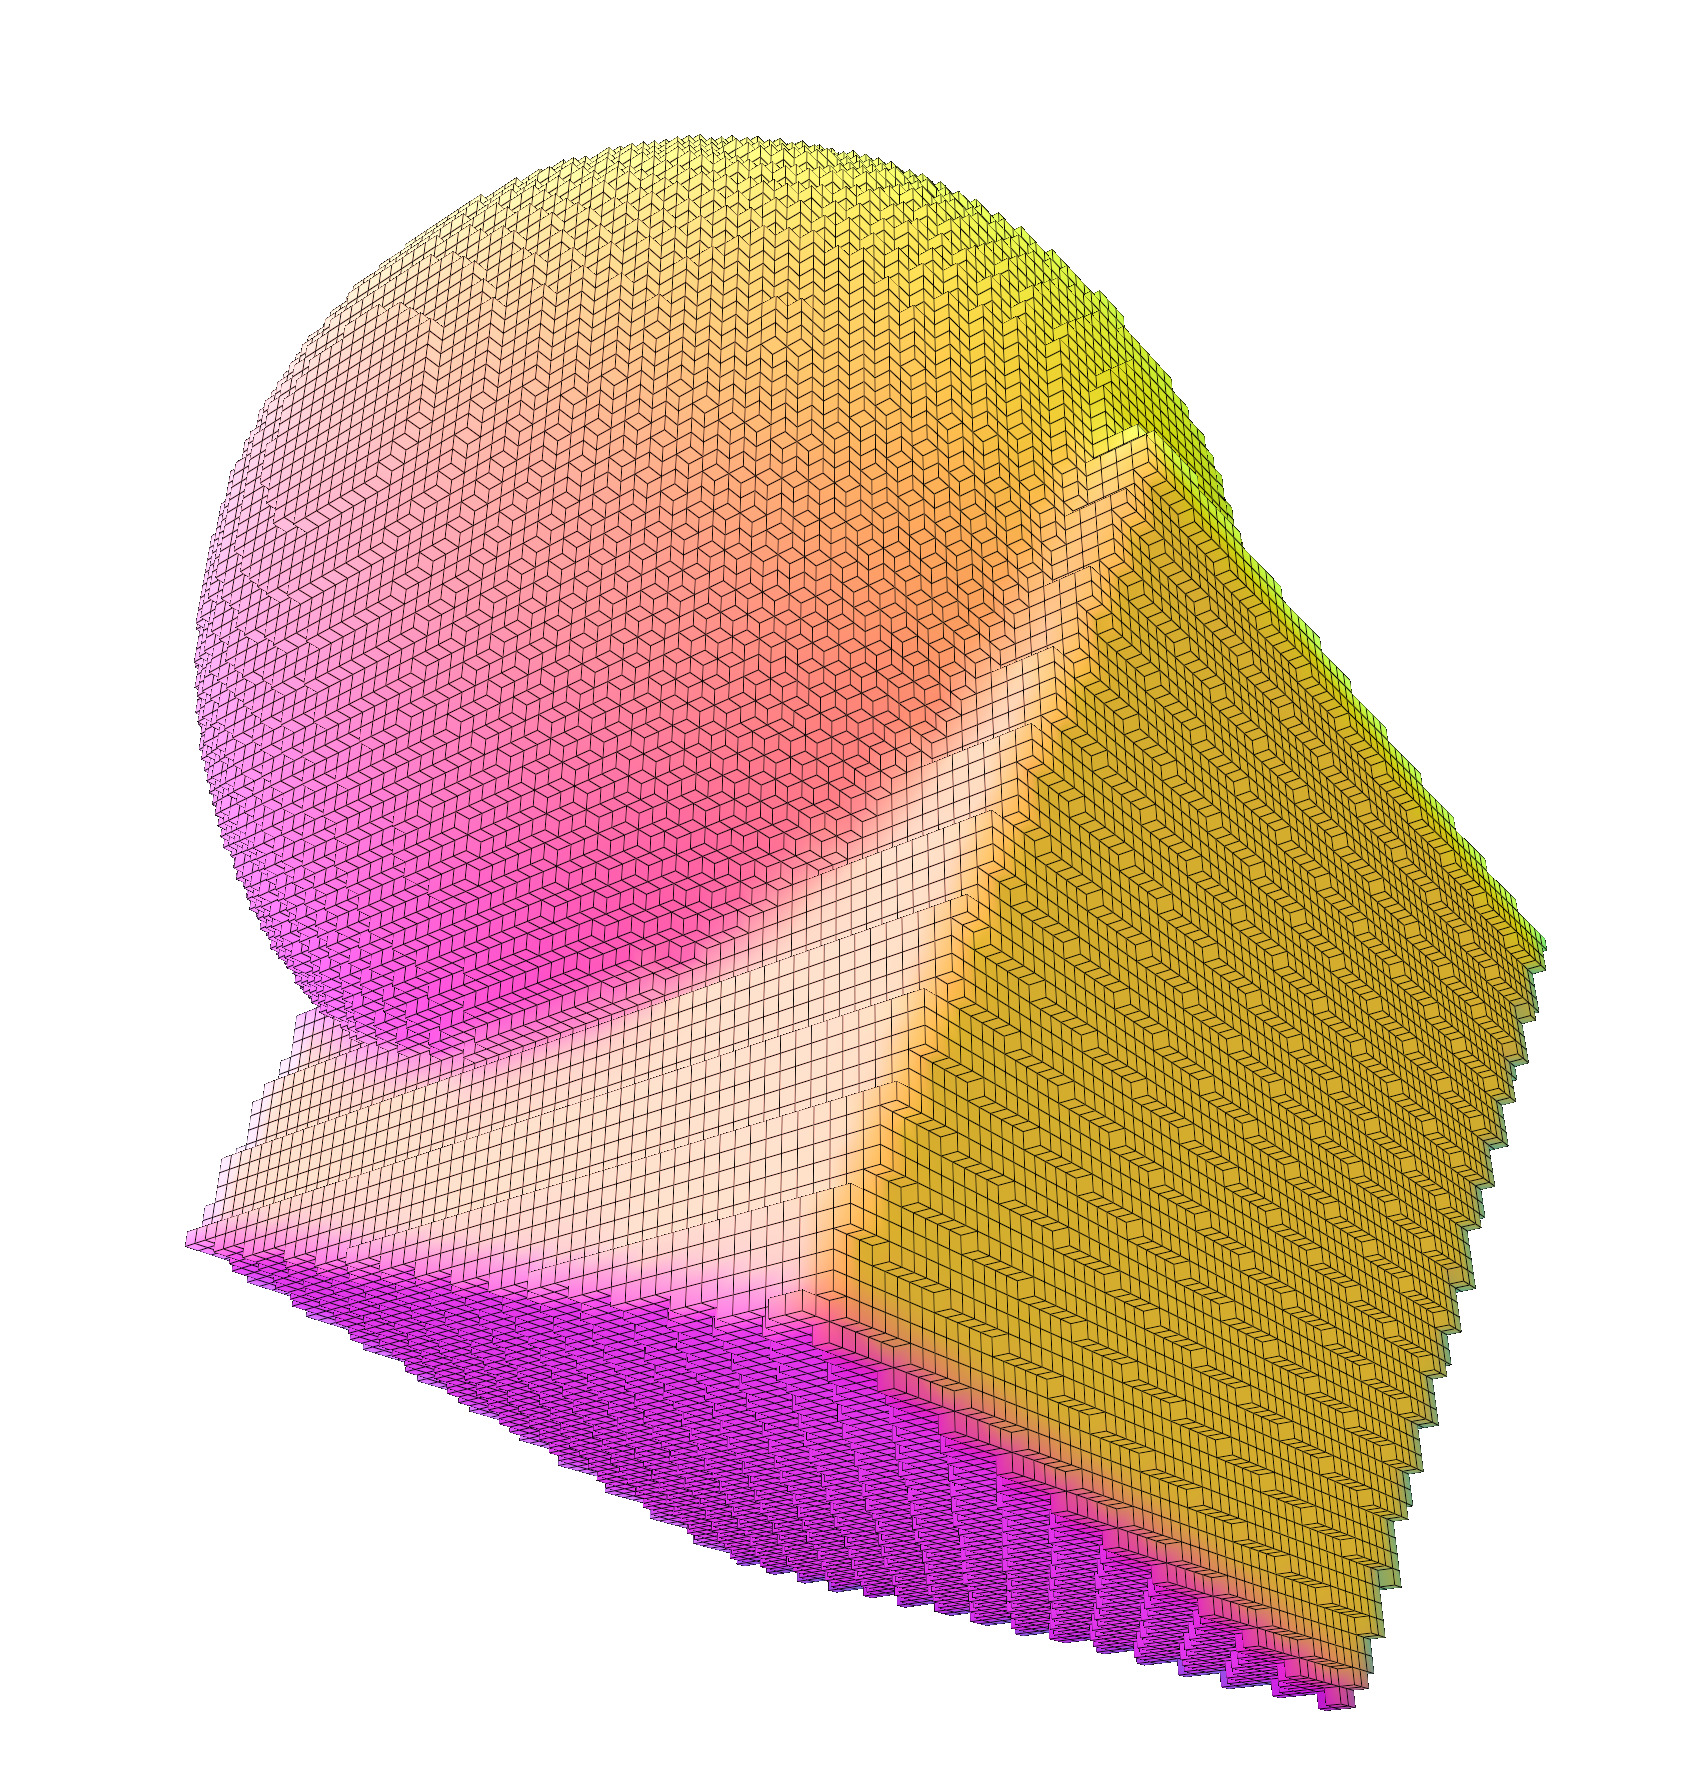
\includegraphics[width=0.3\textwidth]{pictures/cps-VN-flat-edge} &
        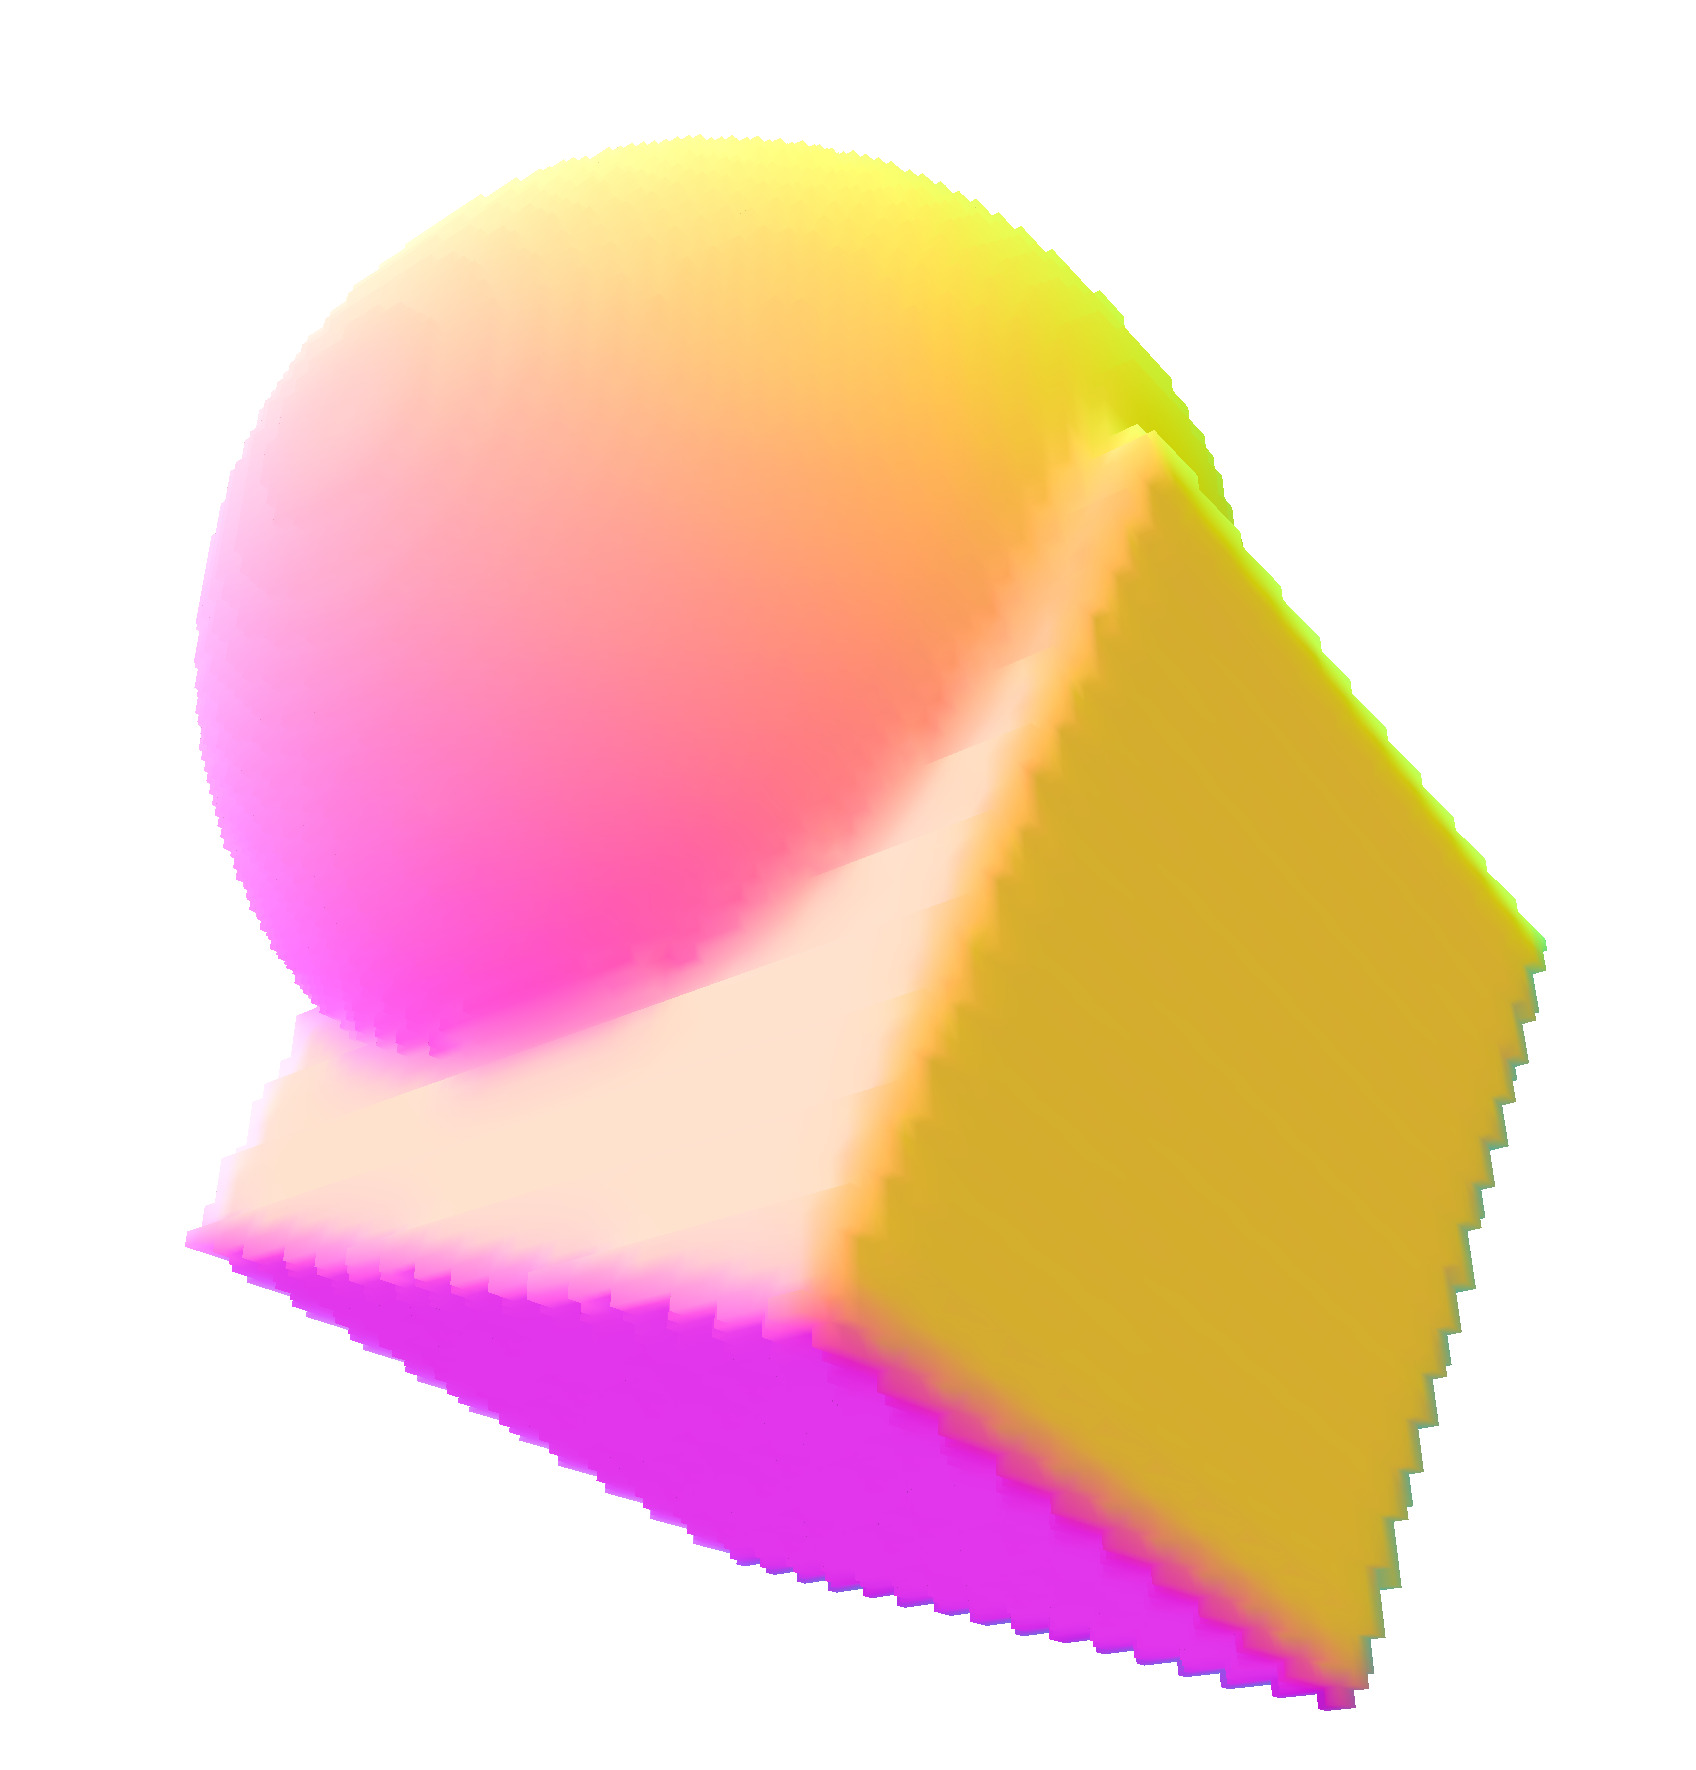
\includegraphics[width=0.3\textwidth]{pictures/cps-VN-flat} \\
        %% 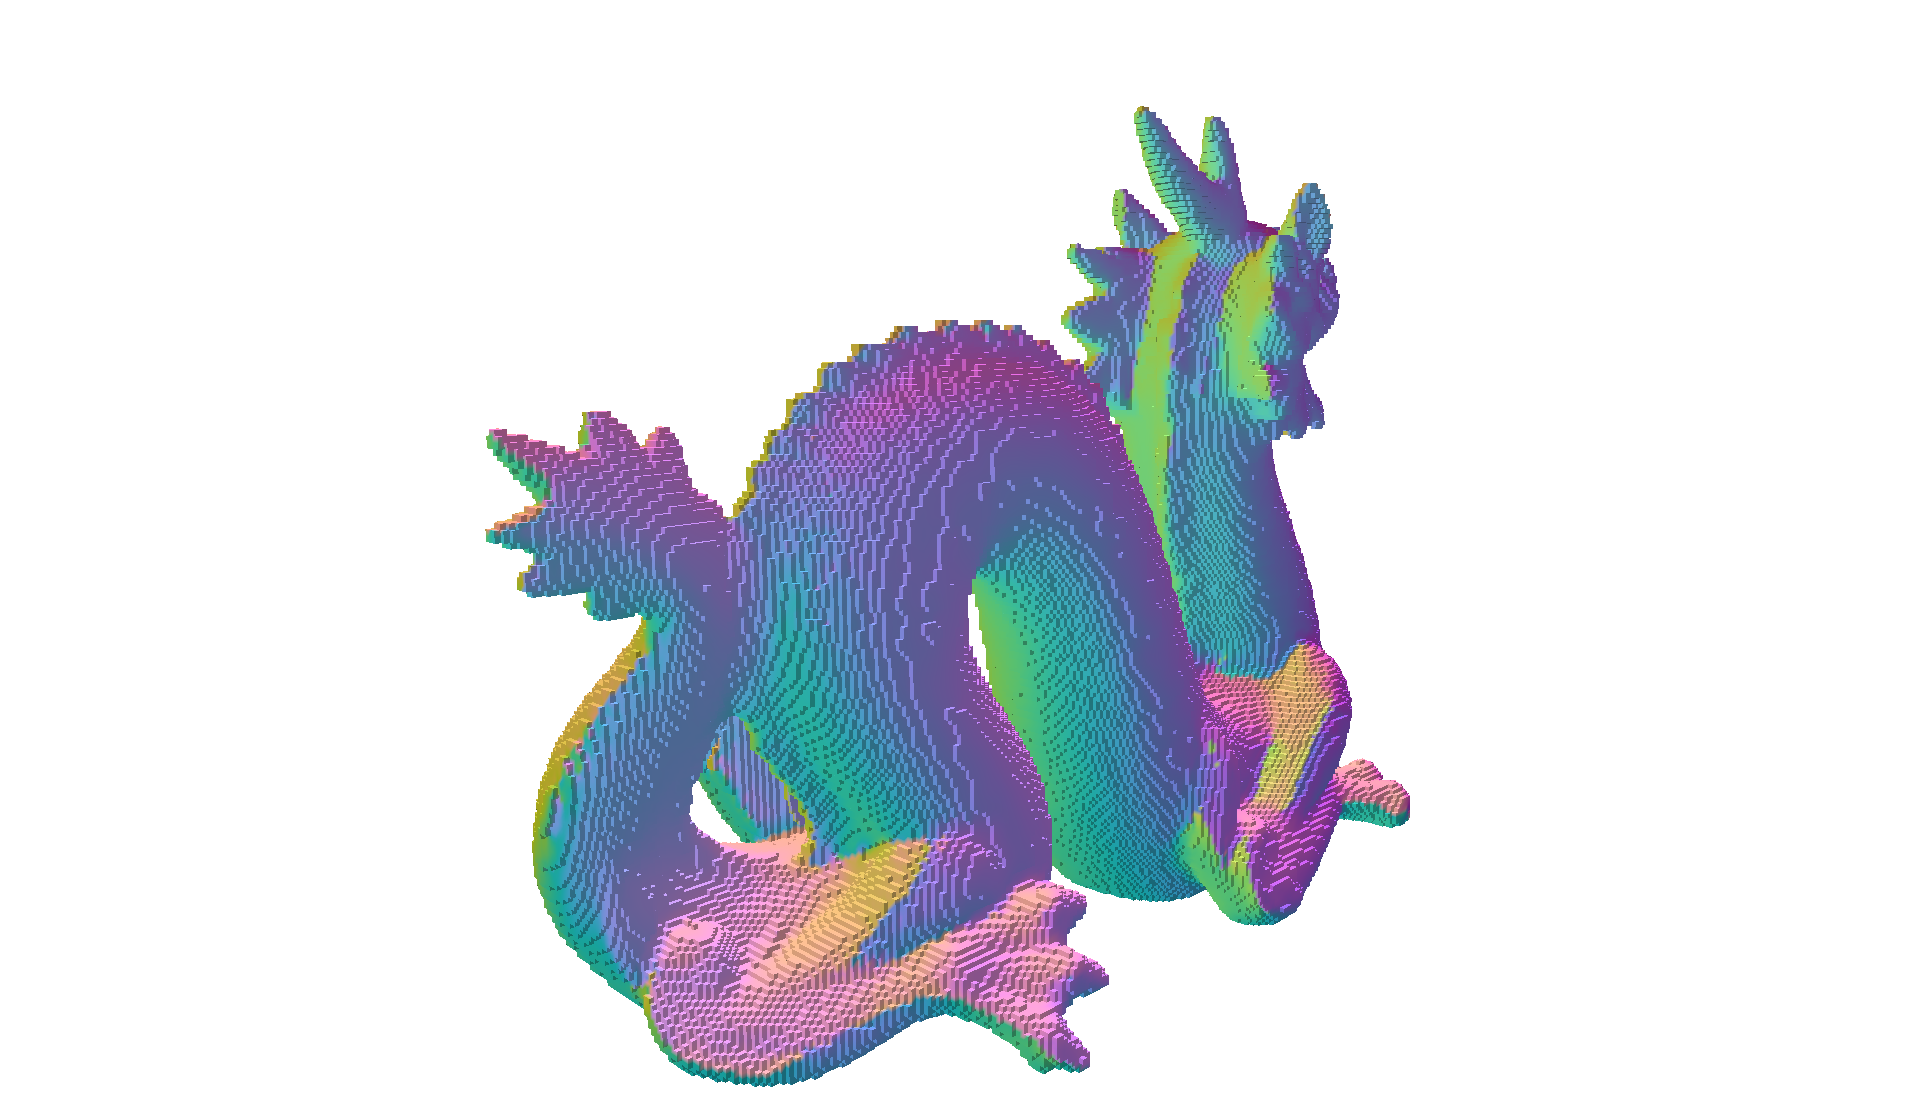
\includegraphics[width=0.4\textwidth]{pictures/chinese-dragon-normal-estimation-cubes-NV} &
        %% 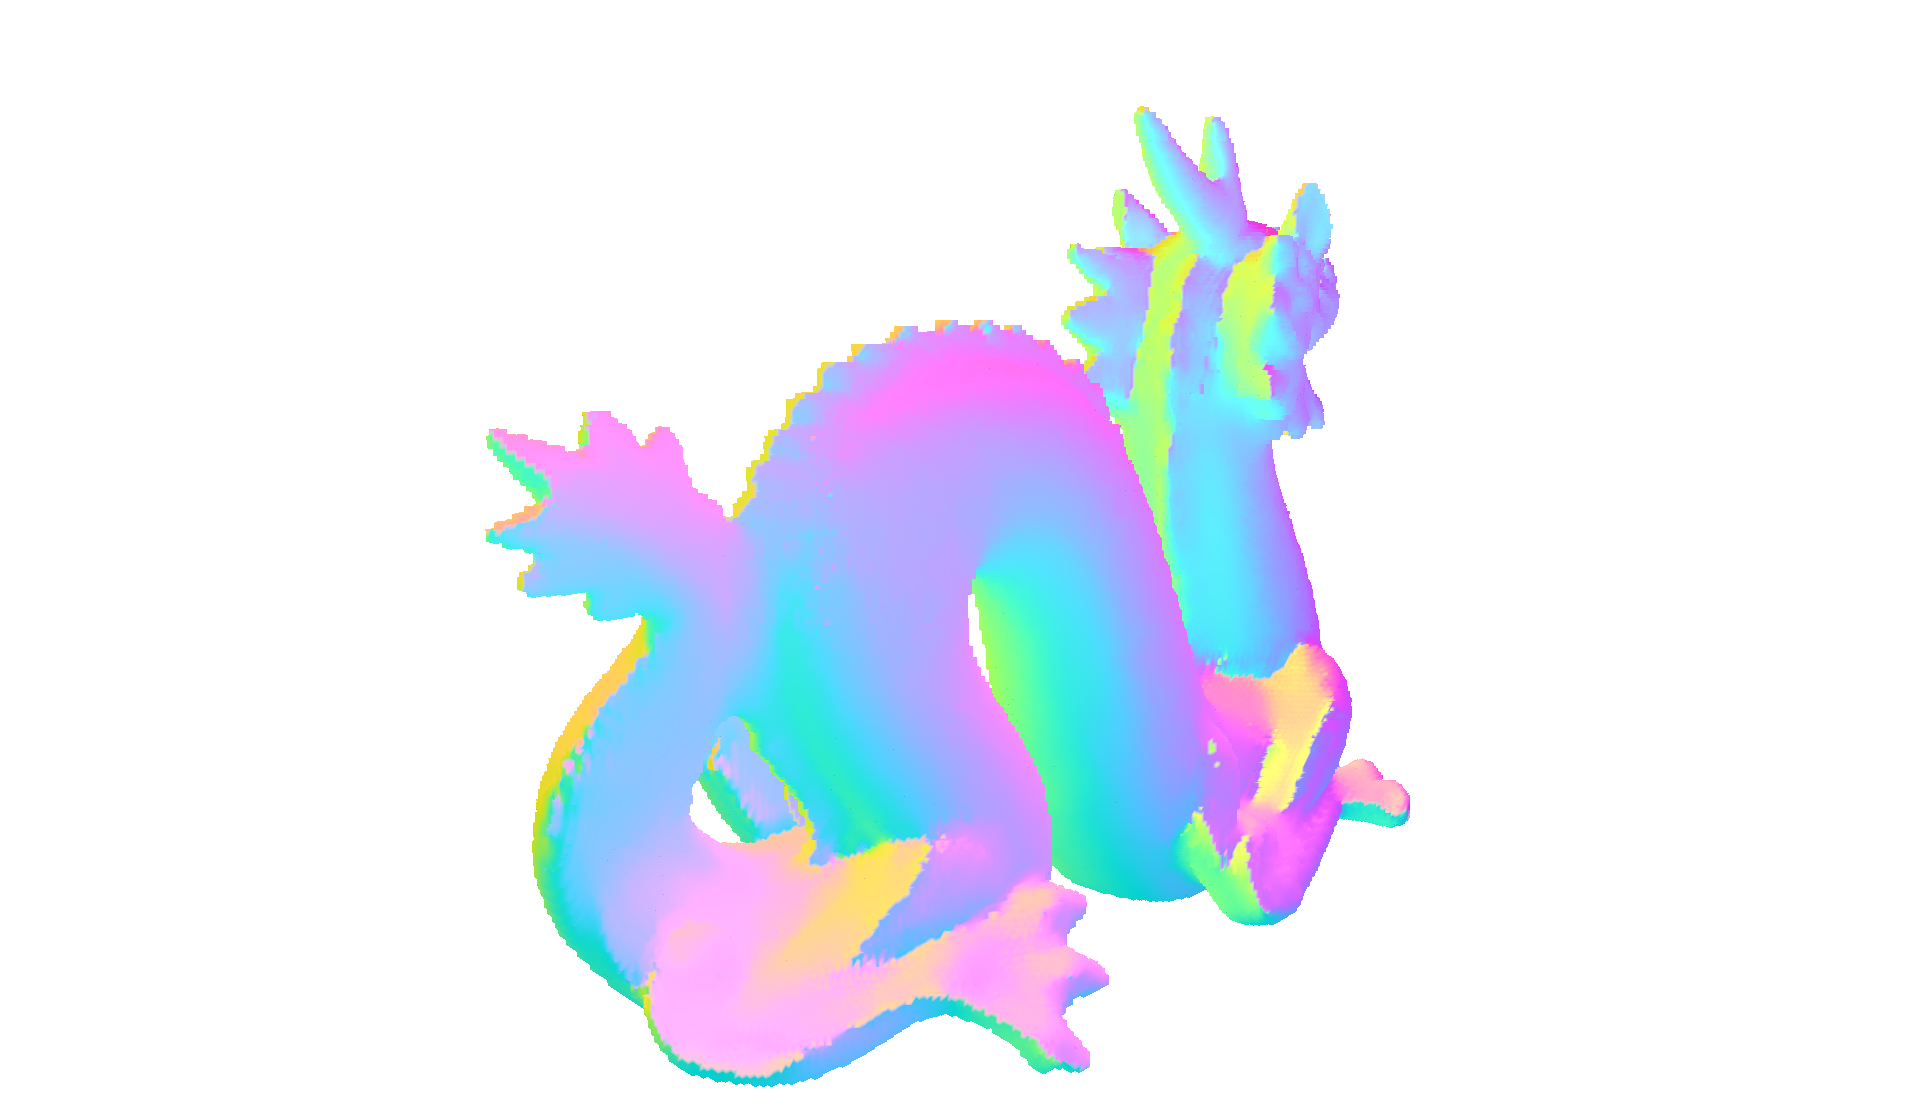
\includegraphics[width=0.4\textwidth]{pictures/chinese-dragon-normal-estimation-smooth-NV} \\
        \hline
        \raisebox{18mm}{II} &
        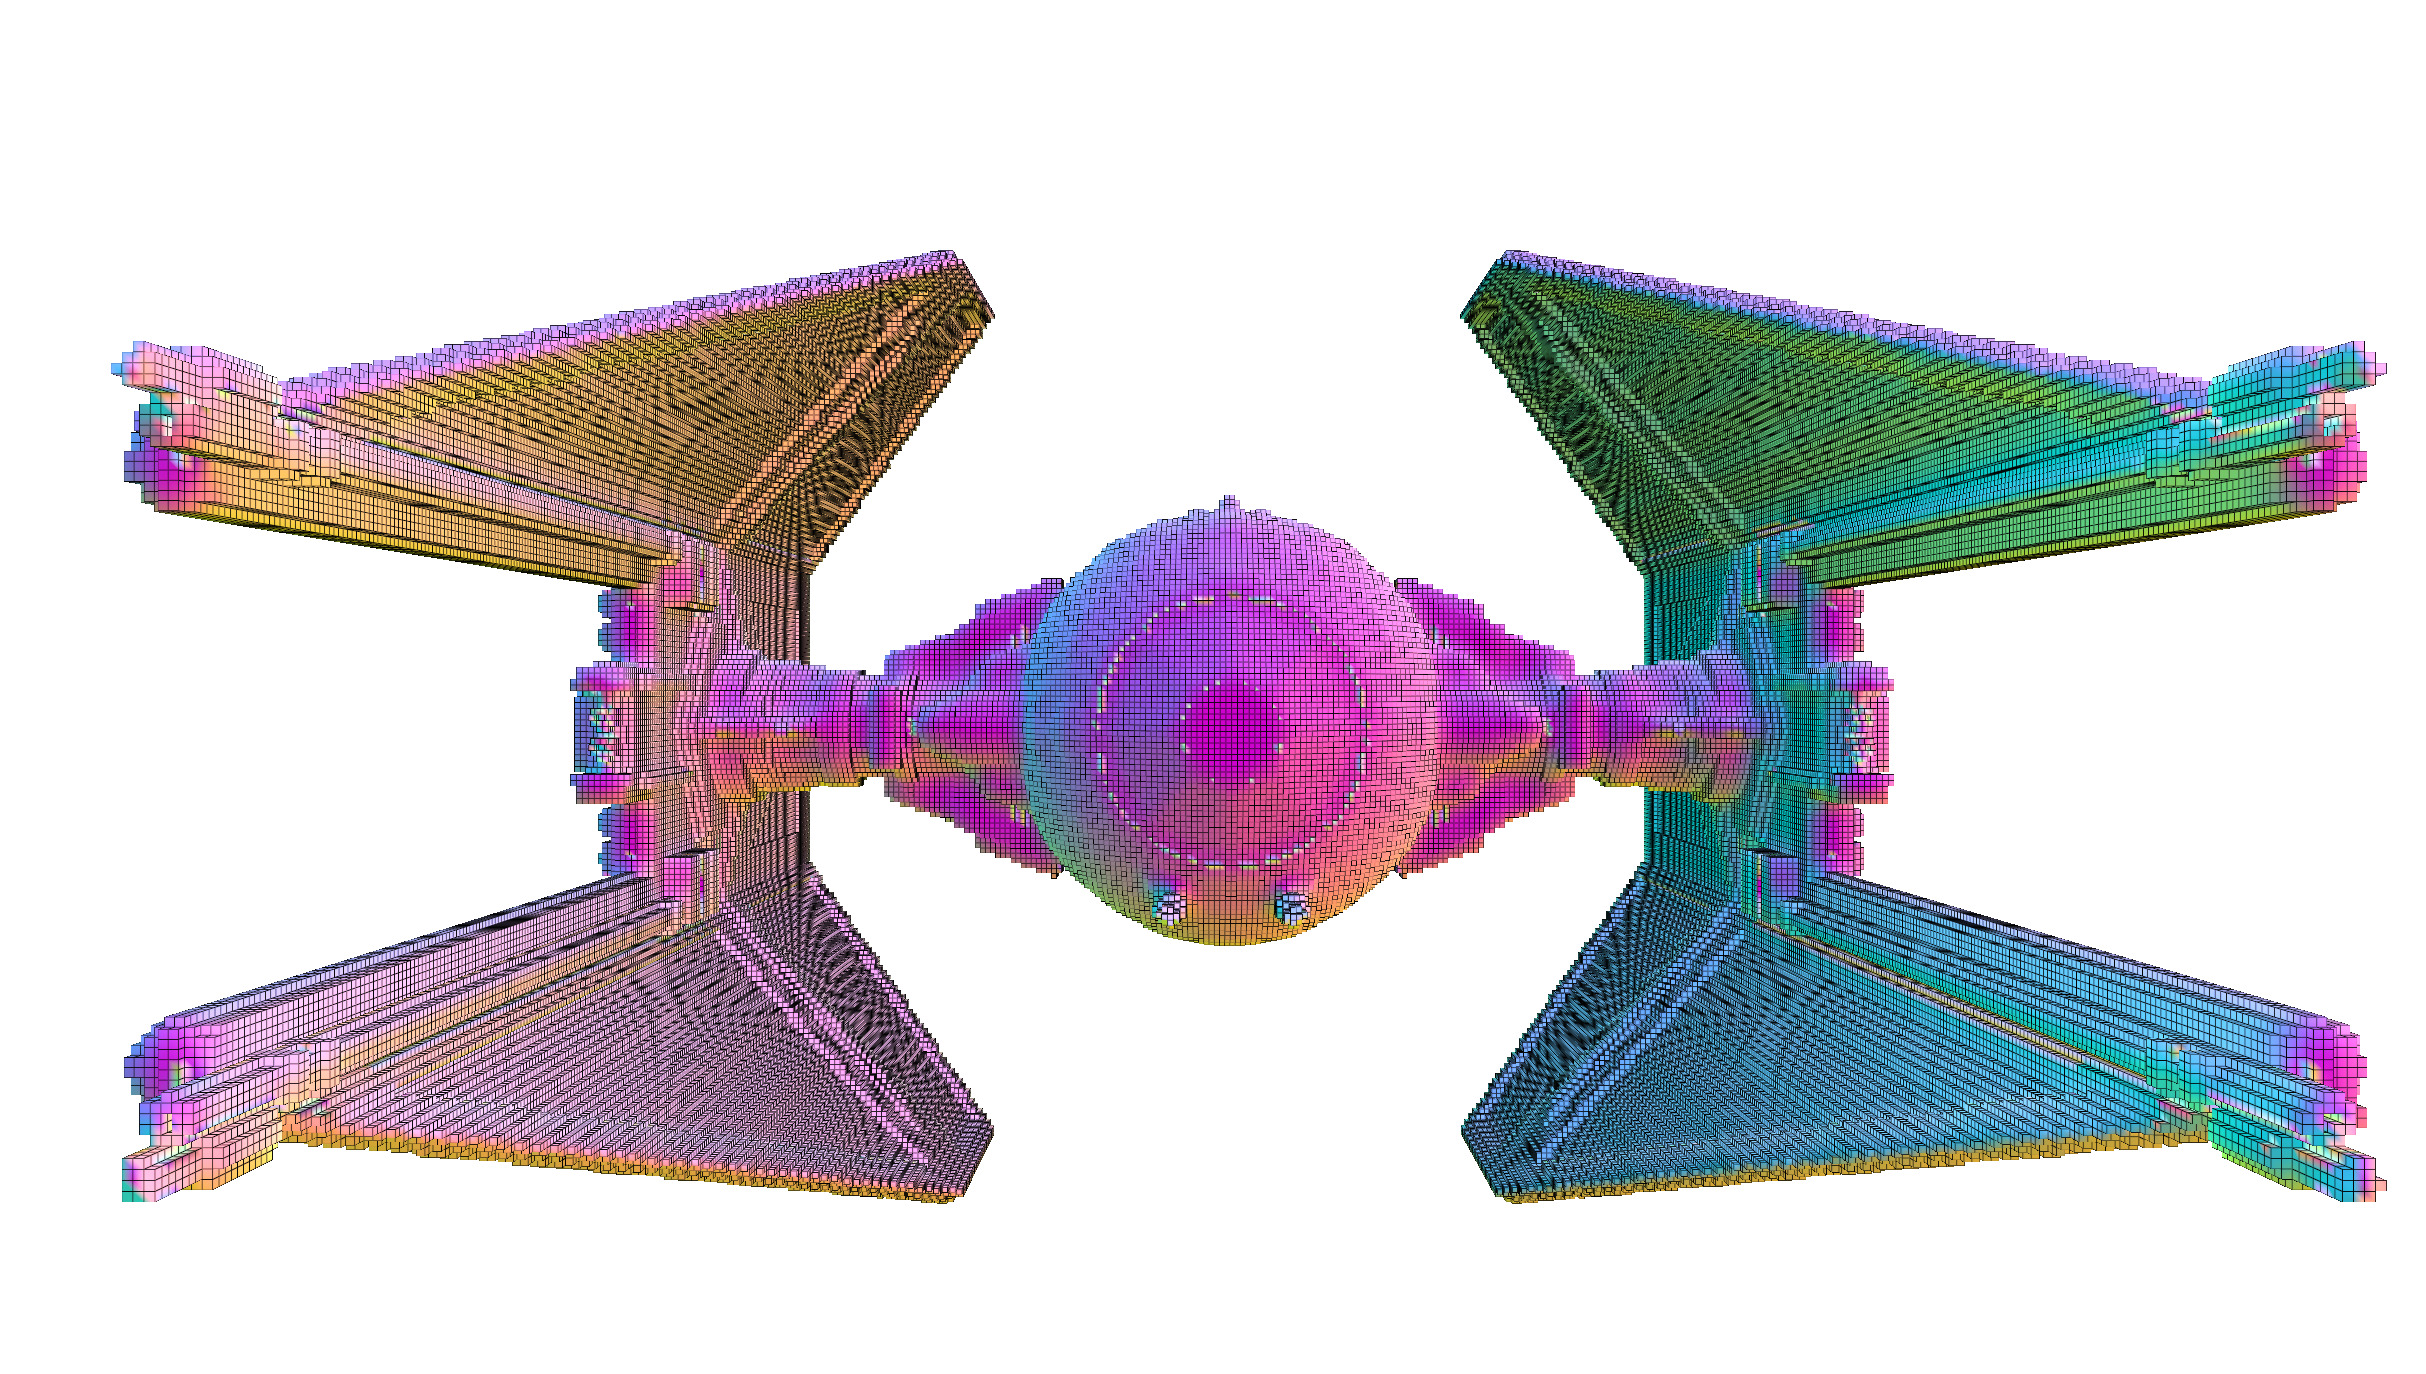
\includegraphics[width=0.43\textwidth]{pictures/tie256-IIN-flat-edge} &
        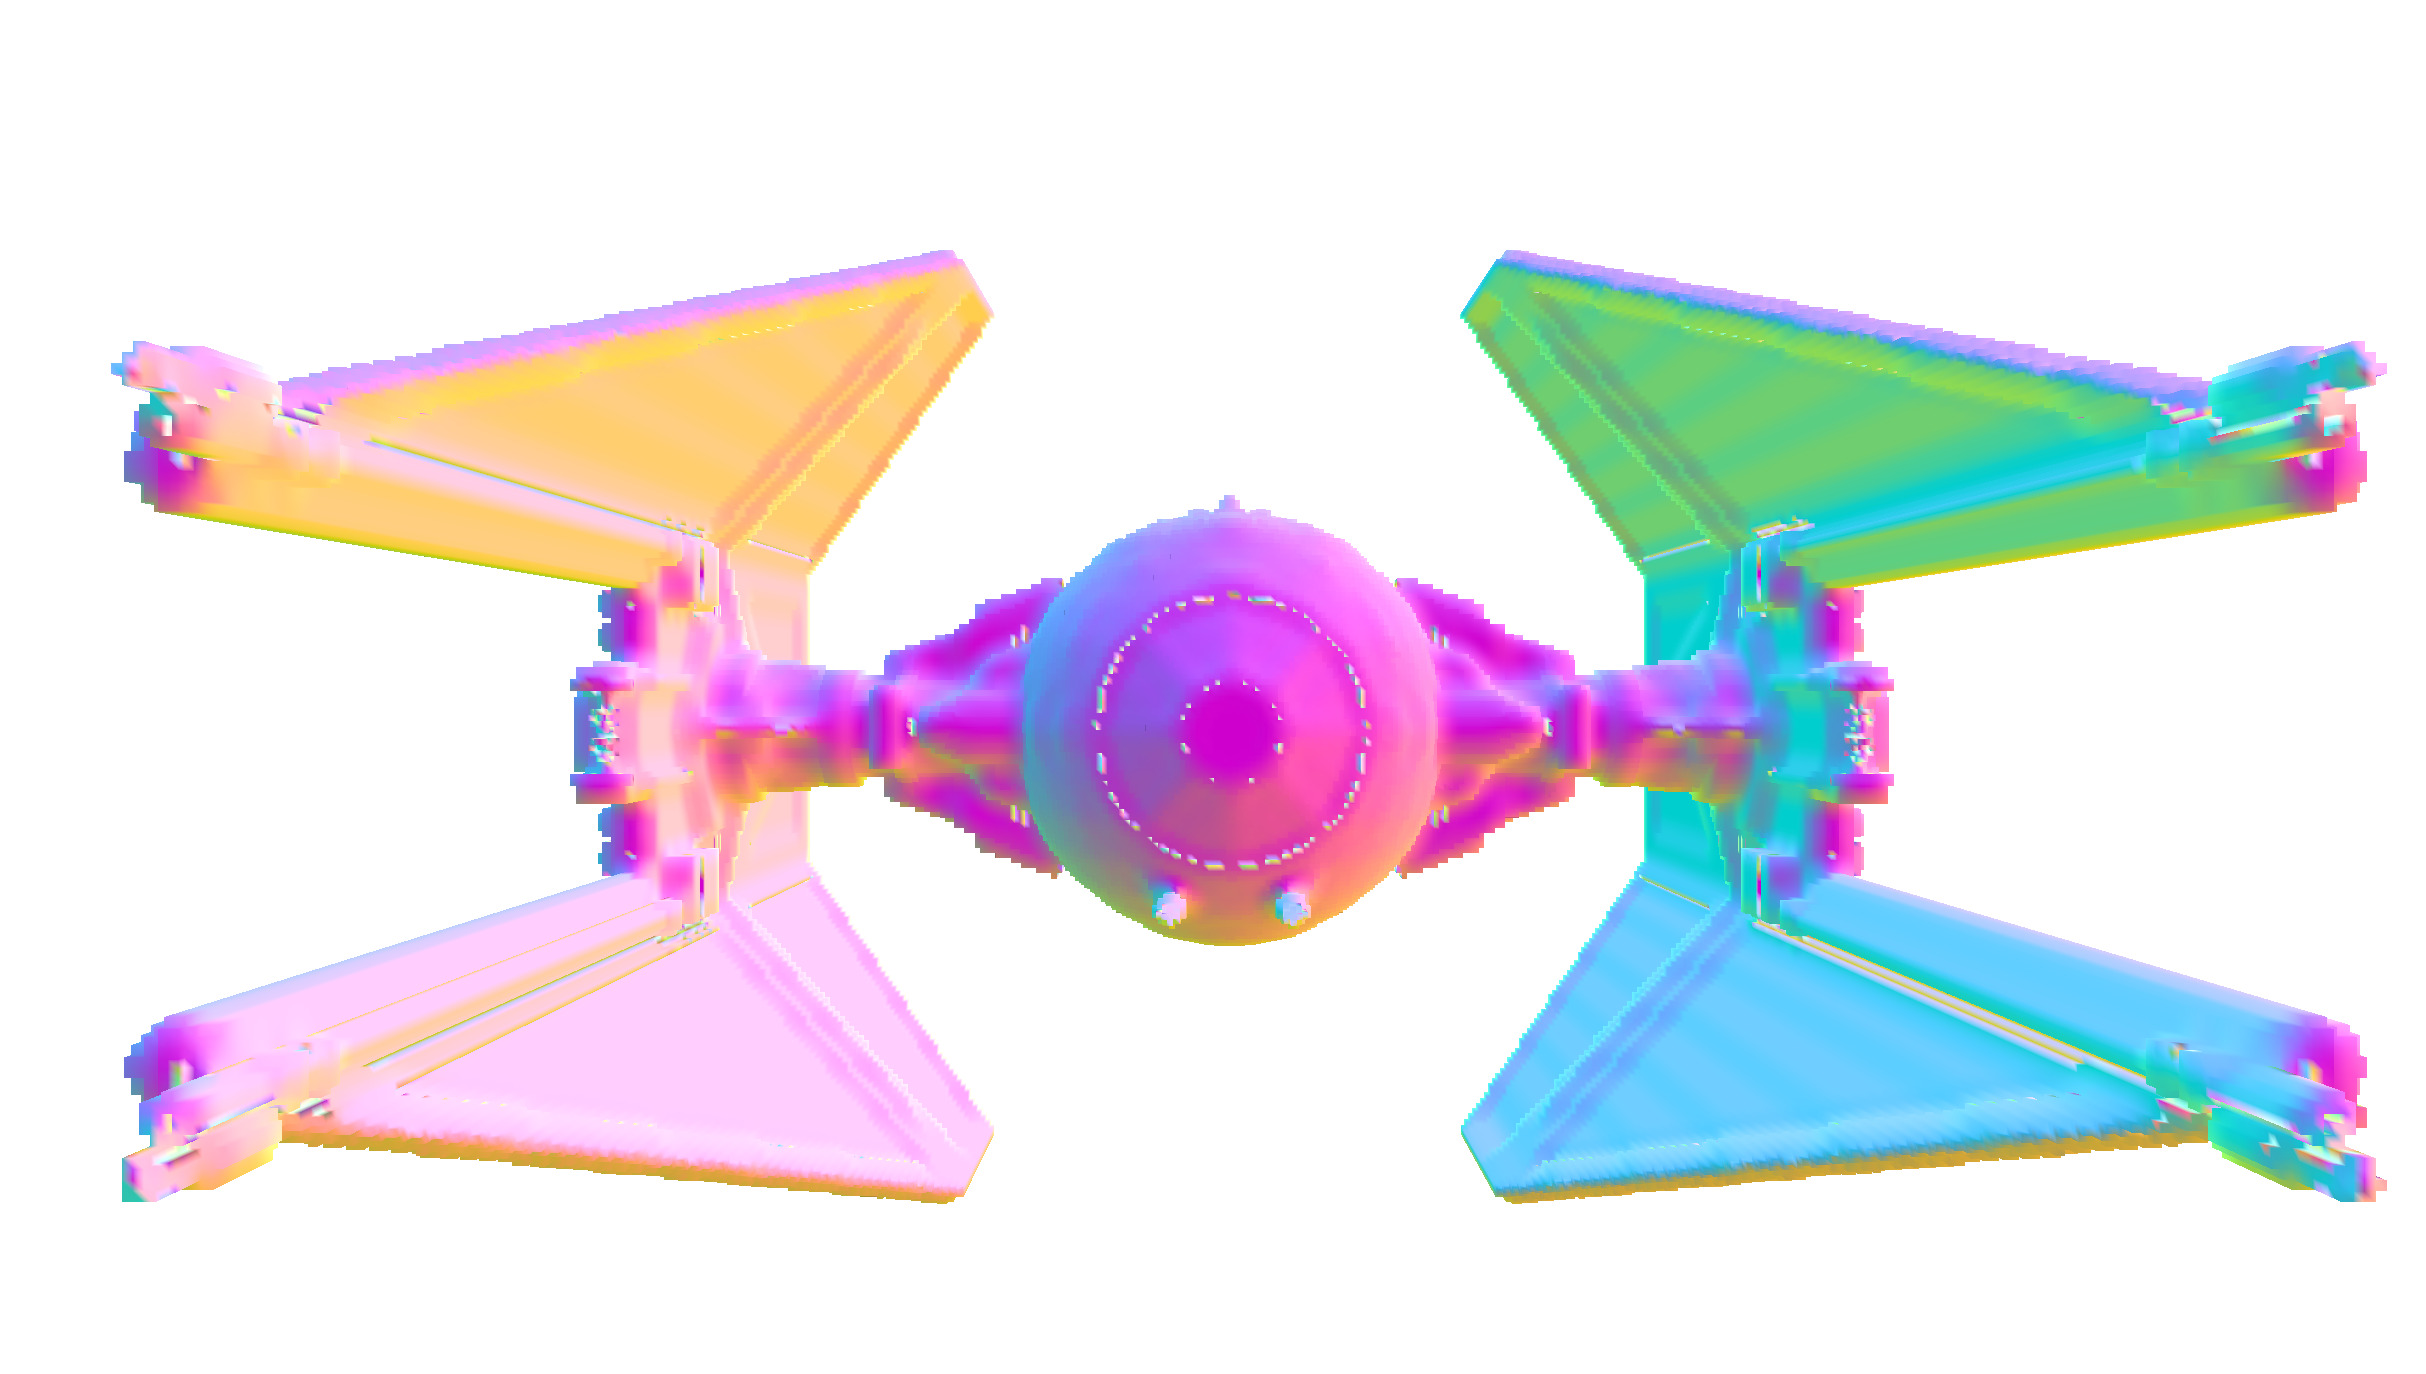
\includegraphics[width=0.43\textwidth]{pictures/tie256-IIN-flat} \\
        %% 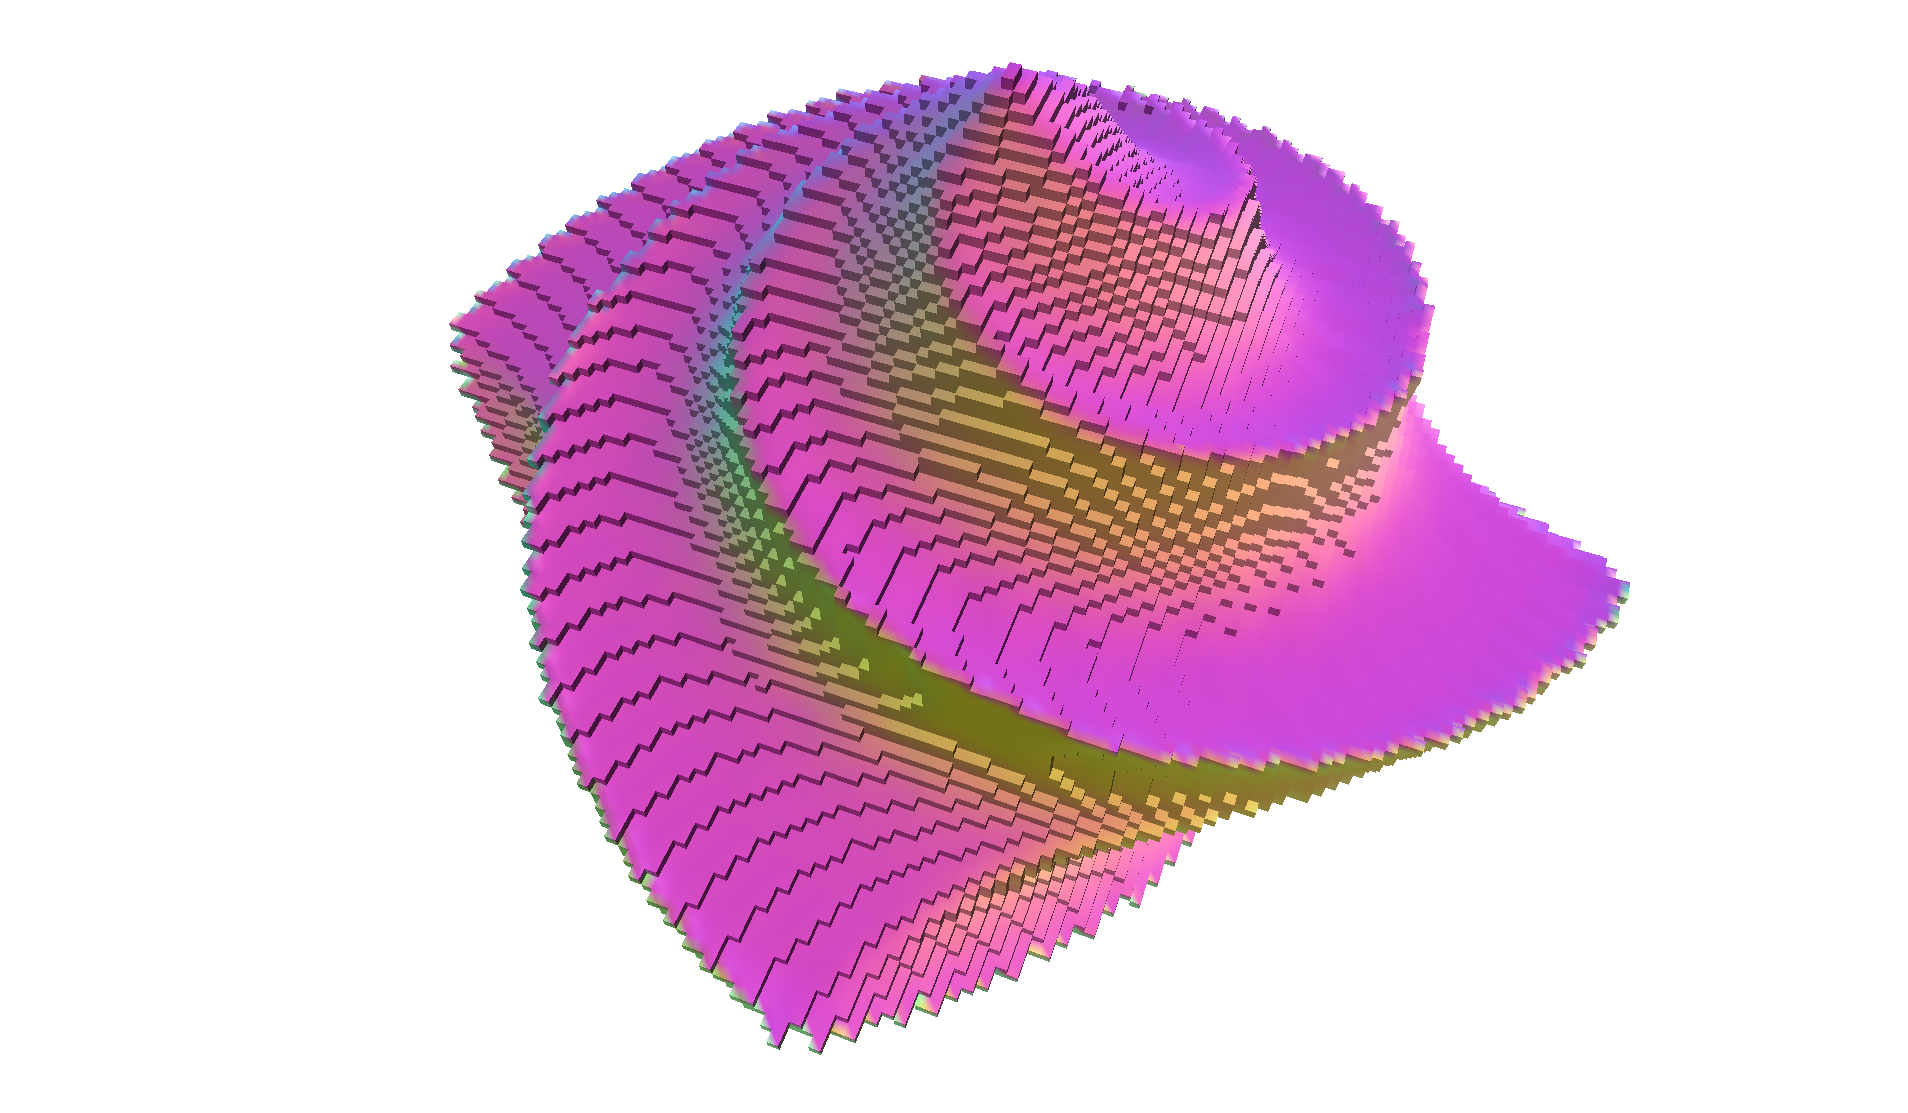
\includegraphics[width=0.4\textwidth]{pictures/octaflower-normal-estimation-cubes-II} &
        %% 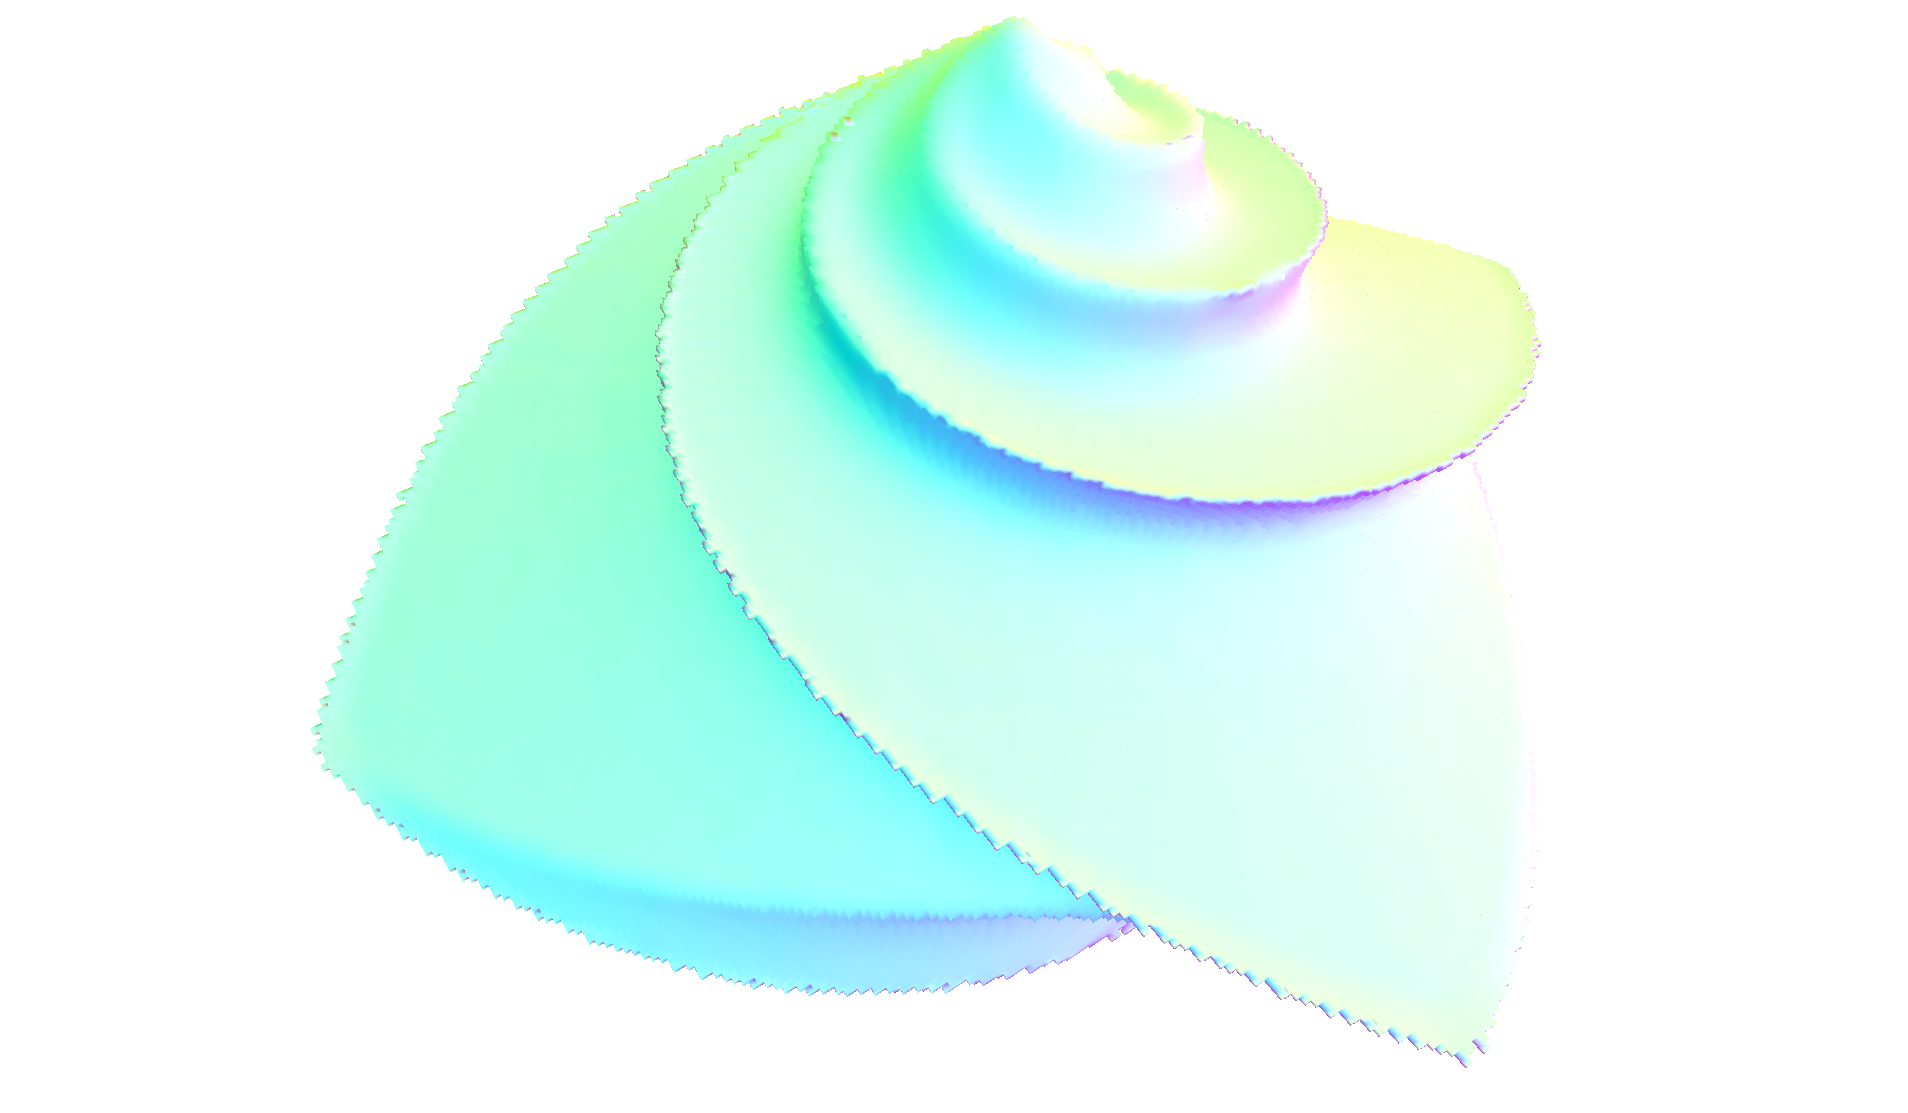
\includegraphics[width=0.4\textwidth]{pictures/octaflower-normal-estimation-smooth-II} \\
        \hline
        \raisebox{18mm}{Ours} &
        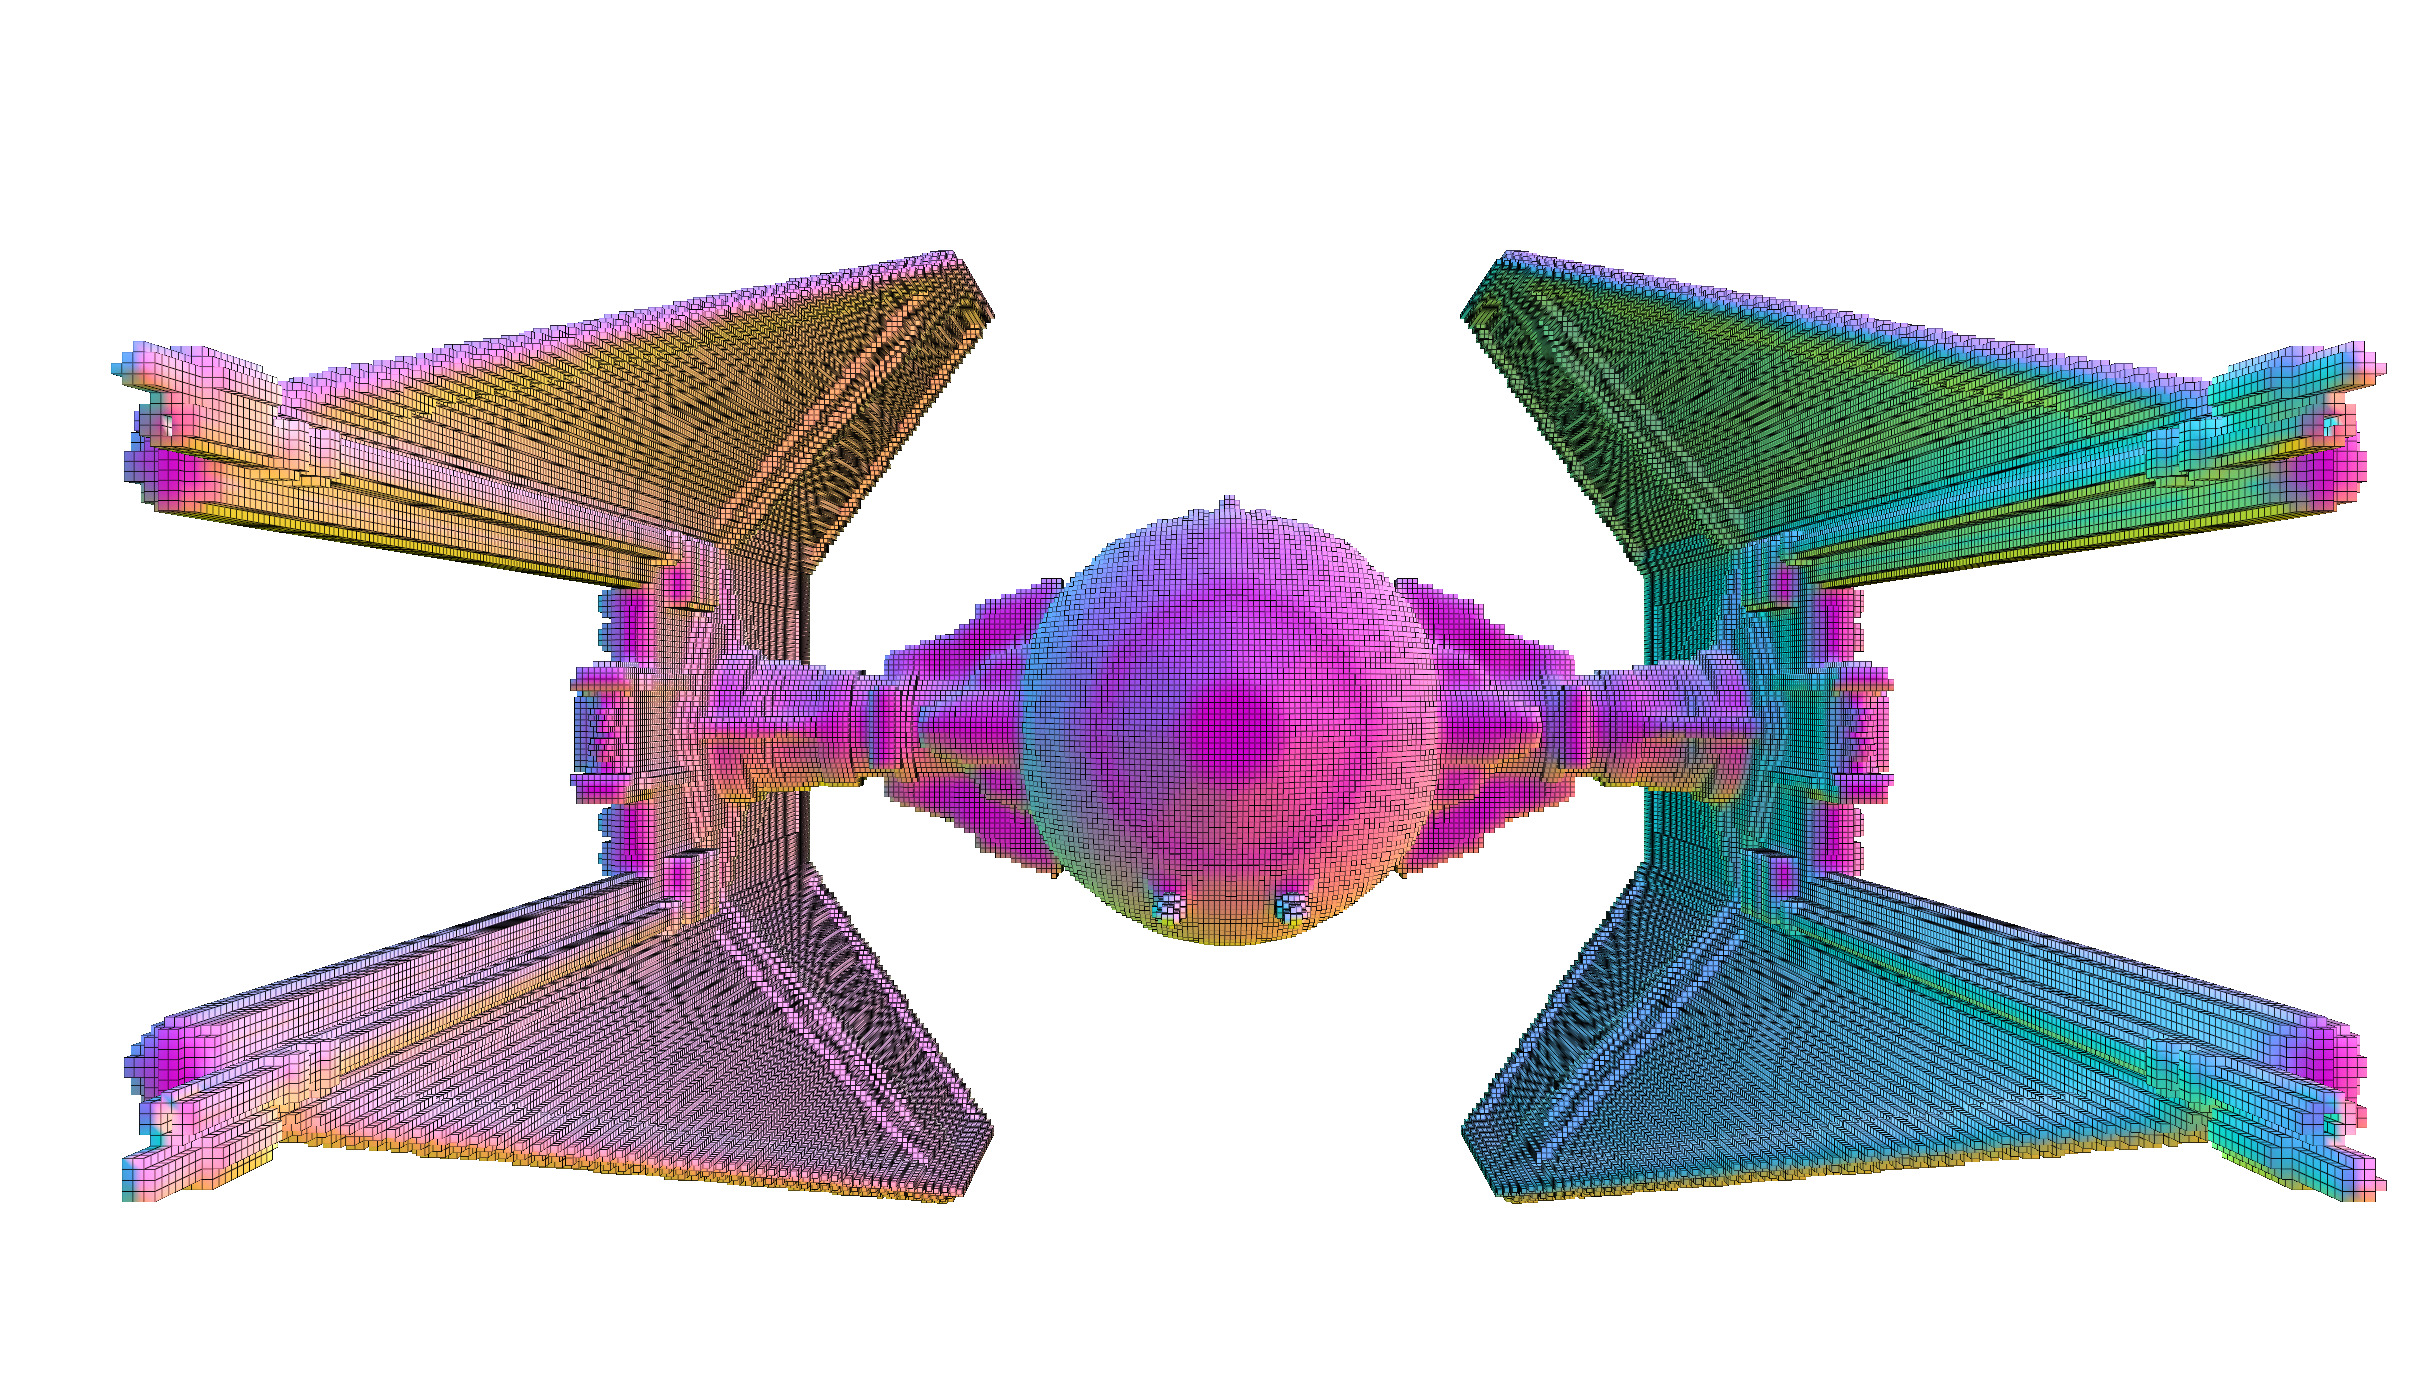
\includegraphics[width=0.43\textwidth]{pictures/tie256-VN-flat-edge} &
        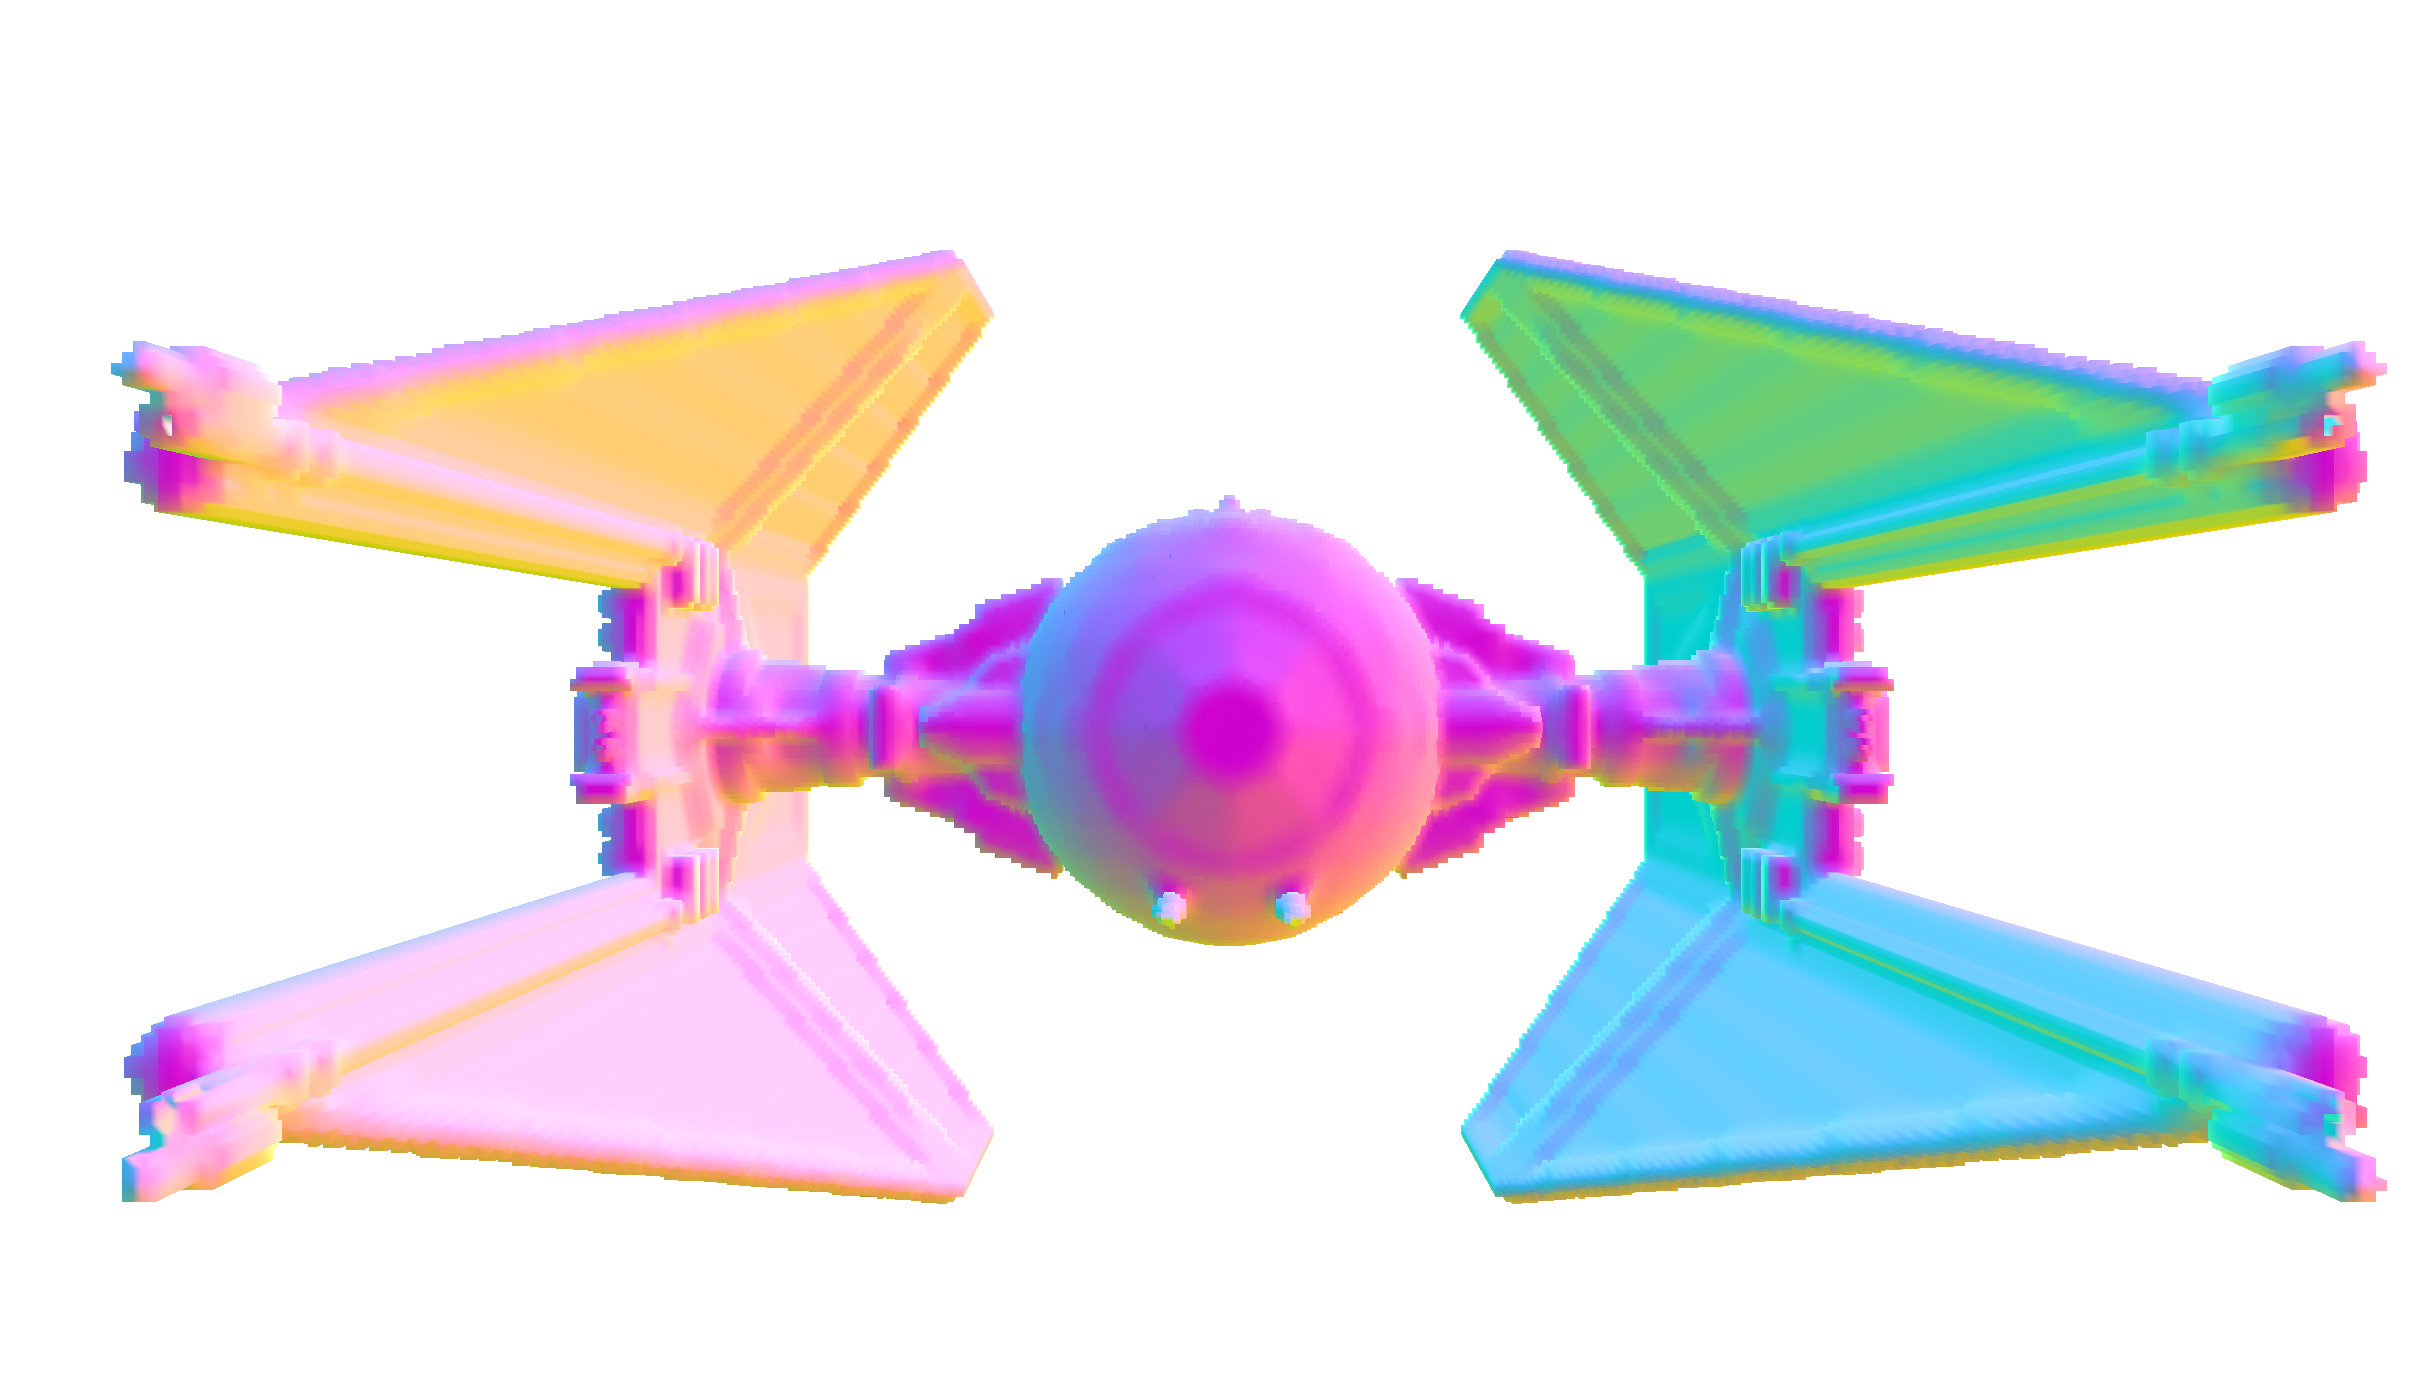
\includegraphics[width=0.43\textwidth]{pictures/tie256-VN-flat} \\
        %% 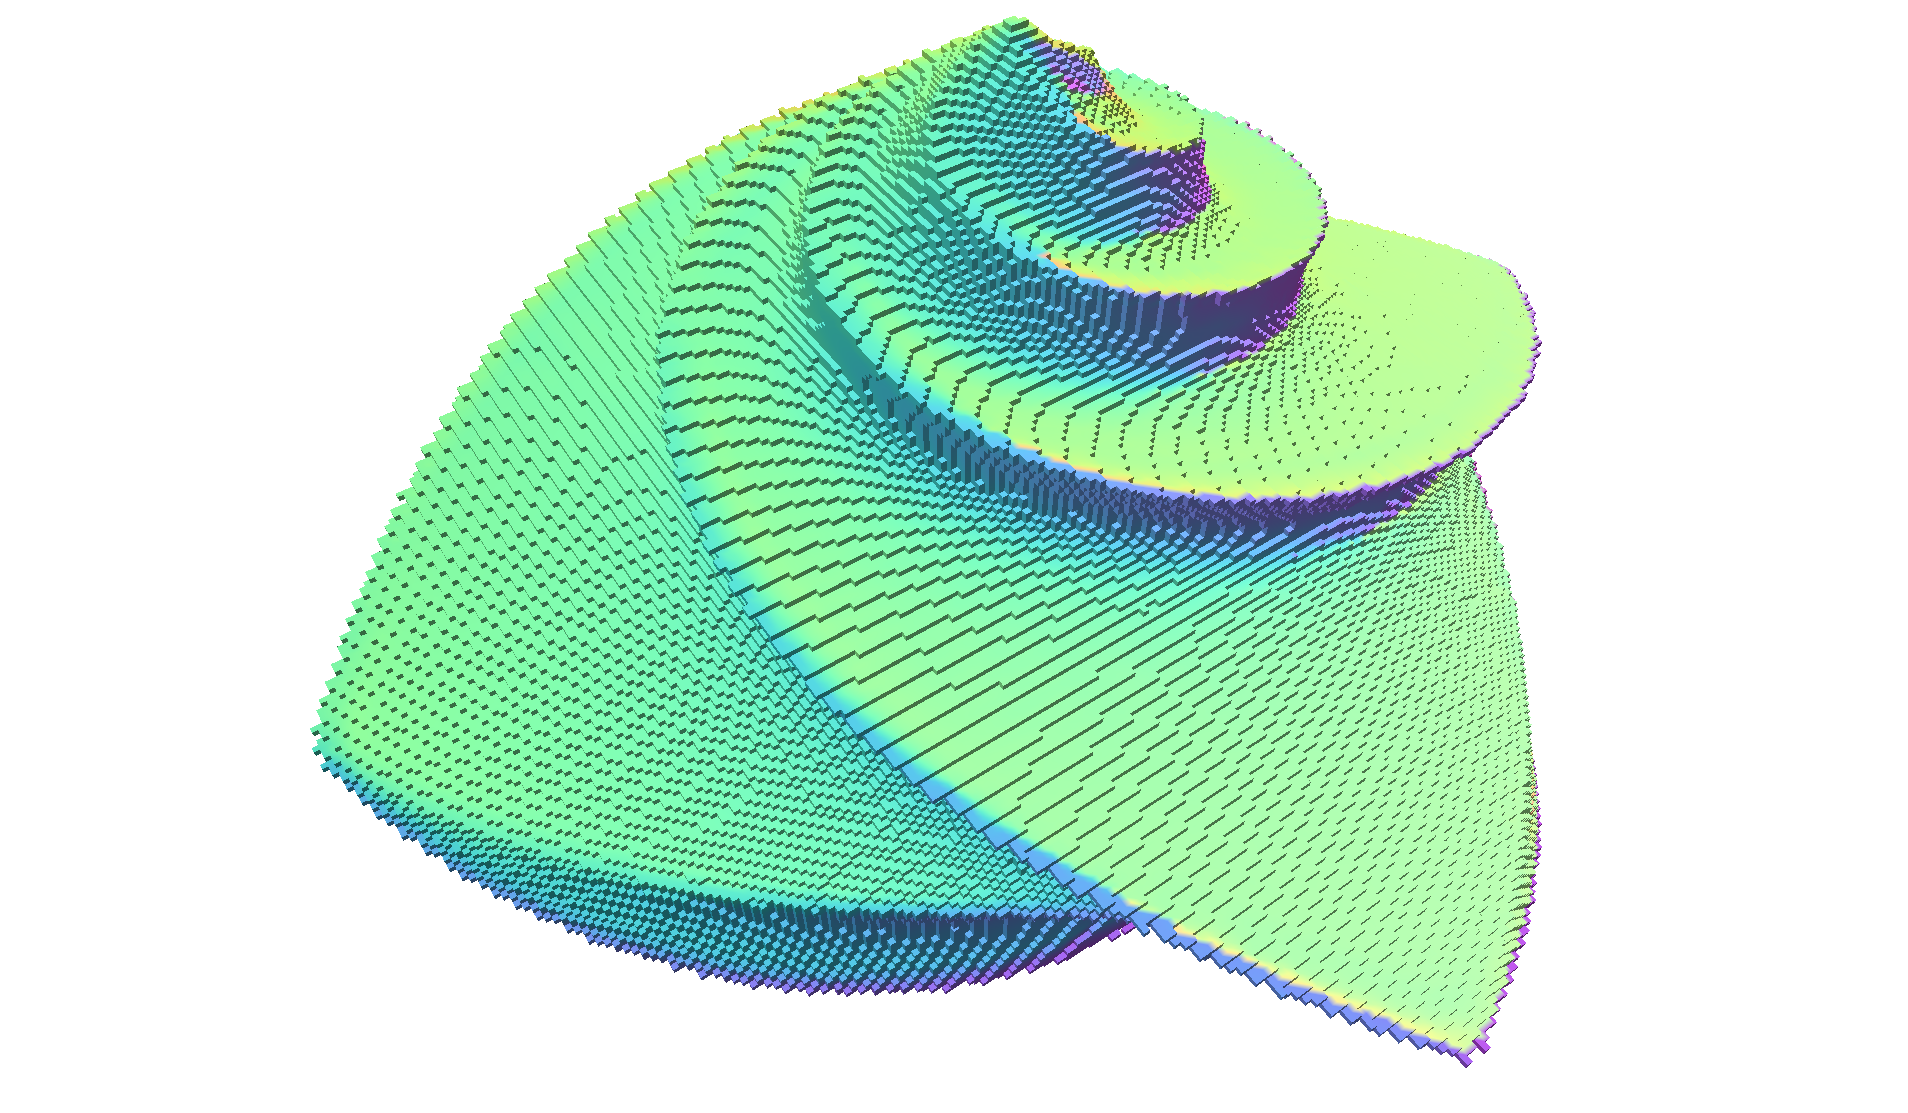
\includegraphics[width=0.4\textwidth]{pictures/octaflower-normal-estimation-cubes-NV} &
        %% 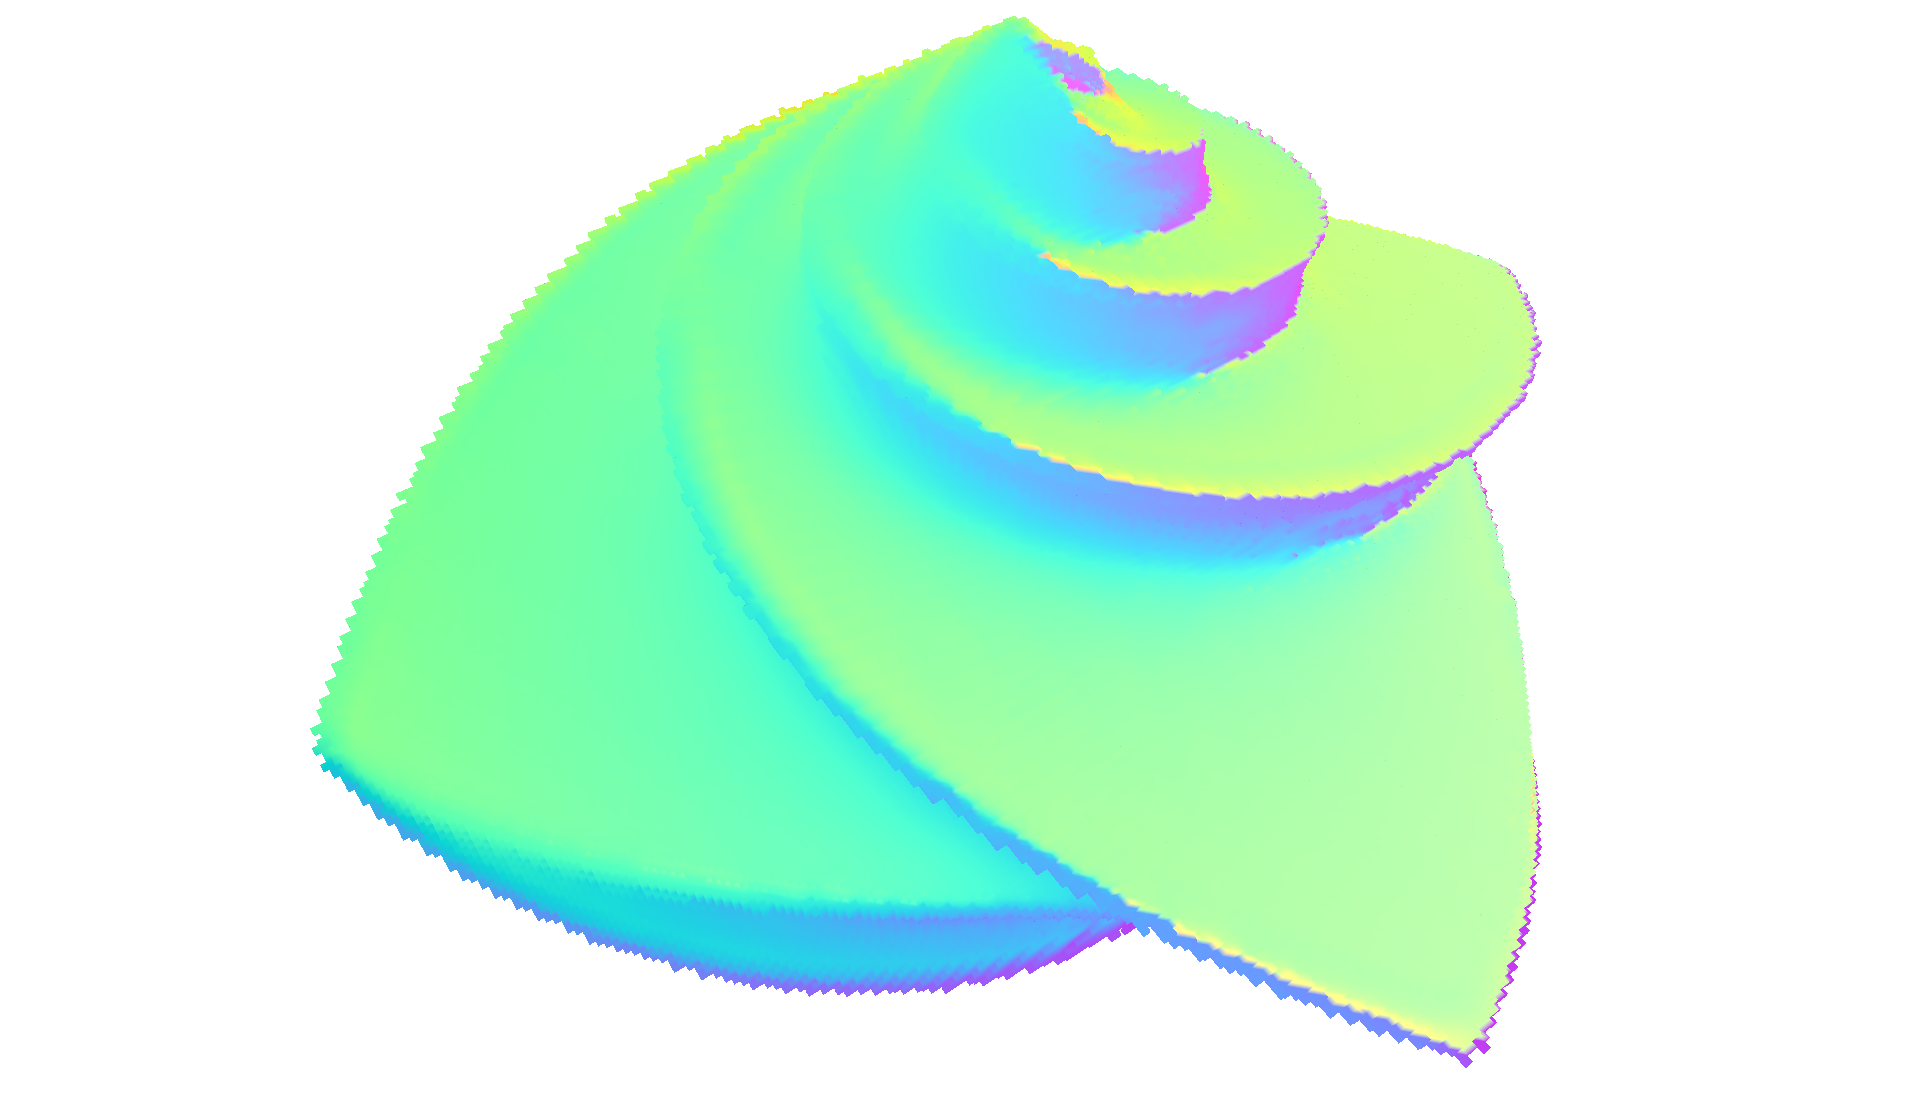
\includegraphics[width=0.4\textwidth]{pictures/octaflower-normal-estimation-smooth-NV} \\
        \hline
    \end{tabular}
    \caption{Examples of normals computed on a cps, then on a
    tie as a color map. First set displays II normals, second set
    uses the visibility algorithm to compute them. The normals are colored
    according to their orientation as $0.5 \cdot (n_i + \mathbbm{1})$. The
    right images are the smooth version of the left images. ``Integral
    Invariant normals'' are computed using a radius of $r=4.5$, while
    our normal estimator are computed using a deviation of $\sigma=4$, and so
    a radius of $r=2\sigma=8$}
    \label{fig:normals-estimation}
\end{figure}

%% Then, to compute the curvatures, we use the Corrected Normal Current
%% estimator~\cite{lachaud:2022-dcg} which are based on the normals computed
%% above.

\paragraph{Application to curvature estimation.}
In order to illustrate better that the visibility normals better
take into account the sharp features of a digital surface while
staying meaningfull in digitization of smooth parts, we compare
the curvature estimates induced by different discrete normal
estimators. We exploit the \emph{Corrected Normal Current (CNC)
    estimator}, whose theory is detailed in~\cite{lachaud:2022-dcg}
and which can estimate all kinds of curvatures given positions and
normals. It produces state-of-the-art curvature estimates on
polygonal surfaces~\cite{lachaud:2020-cgf}, point clouds~\cite{lachaud:2023-cgf}, and even outperforms Integral Invariant
curvature estimates~\cite{coeurjolly:2014-cviu} on digital
surfaces~\cite{lachaud:2022-dcg}. Its implementation is also
available in    \href{https://dgtal-team.github.io/doc-nightly/moduleCurvatureMeasures.html}{\textsc{DGtal}}.

Figure~\ref{fig:fig-curvatures} displays the results of CNC curvature
estimations on the digitization of a piecewise smooth shape
``Talking D20'', taken from
\href{https://ten-thousand-models.appspot.com/detail.html?file_id=1533028}{Thingi10K}.
We compare the differences obtained by just changing the discrete
normal estimator (available in the \textsc{DGtal} library):
(column II normals) Integral Invariant normals with $r=6$, (column
CTriv normals) convolved trivial normals with $r=6$, (column
Visibility normals) our proposed estimator (VN) with $\sigma=4$ and
maximal visibility distance $2\sigma$. These parameters were
chosen so that the respective computation windows of the different
estimators are approximately the same.

The II estimator is good along digitization of smooth or flat parts of
the dice, but presents curious artefacts near sharp features
induced by the hollowed out numbers: this is due to the nature of
II normal estimates, which computes a PCA of a ball centered on
the point of interest and may include points on the other side of
the saliencies.

The CTriv estimator only performs averaging of trivial normal
directions along the surface. It behaves much better than II near
features (although it tends to smooth curvatures) since it does
not use information from across the gap. However some oscillations
of the curvatures are distinguishable especially along the flat
parts, and some curvature estimates are erroneous on smoother
parts (like the edge above 6 for $\kappa_2$ or several dice
vertices).

The VN estimator takes the best of the two previous approaches. It
remains precise and stable on smooth and flat regions, while
perfectly delineating sharp features and holes, whatever the kind
of estimated curvatures. Its drawback is the computation time,
which is $52s$ for a maximal visibility distance $8$, compared to
$2.3$s for II and $0.1s$ for CTriv. Note that the computation time
falls back to $33s$ for a maximal distance of $6$ (and same
$\sigma=4$) while the result is visually indistinguishable.


\newcommand{\MyZoom}[1]{%
    \begin{tikzpicture}[spy using outlines={circle,magnification=1.8,size=2cm,connect spies}]
    \node[inner sep=0pt] {\pgfimage[width=0.3\textwidth]{#1}};
    \spy[overlay,blue] on (0.4,0.2) in node at (-0.8,0.8);
    \end{tikzpicture}}
% \newcommand{\MyZoom}[1]{\includegraphics[width=0.3\textwidth]{#1}}

\begin{figure}
    \begin{center}
        \begin{tabular}{|c||c|c|c|}
            \hline
            Curv. & II normals & CTriv normals & Our normals \\ \hline \hline
            \raisebox{18mm}{$\kappa_1$} &
            \MyZoom{pictures/d20-k1-II.jpg} &
            \MyZoom{pictures/d20-k1-CTriv.jpg}&
            \MyZoom{pictures/d20-k1-VN.jpg}\\ \hline
            \raisebox{18mm}{$\kappa_2$} &
            \MyZoom{pictures/d20-k2-II.jpg} &
            \MyZoom{pictures/d20-k2-CTriv.jpg}&
            \MyZoom{pictures/d20-k2-VN.jpg}\\ \hline
            \raisebox{18mm}{$H$} &
            \MyZoom{pictures/d20-H-II.jpg} &
            \MyZoom{pictures/d20-H-CTriv.jpg}&
            \MyZoom{pictures/d20-H-VN.jpg}\\ \hline
            \raisebox{18mm}{$G$} &
            \MyZoom{pictures/d20-G-II.jpg} &
            \MyZoom{pictures/d20-G-CTriv.jpg}&
            \MyZoom{pictures/d20-G-VN.jpg}\\ \hline
        \end{tabular}
    \end{center}
    \caption{\label{fig:fig-curvatures}Estimation of curvatures using
    Corrected Normal Current estimators \cite{lachaud:2022-dcg}
    with a measure of radius $2$ for the shape ``Dice-20'' of
    Thingi10K database at resolution $256^3$. This estimator is
    parameterized by an input normal estimator: first column by
    ``Integral Invariant normals'' (radius $r=6$), second column
    by ``Convolved Trivial normals'' (radius $k=6$), third
    column by our presented normal estimator (deviation
        $\sigma=4$, radius $r=2\sigma=8$). Per row are displayed the
        estimated curvatures in order: first and second principal
        curvatures $\kappa_1$ and $\kappa_2$, mean curvature $H$,
        Gaussian curvature $G$. The range of curvature between deep
        blue and deep red is $\lbrack -0.1, 0.1 \rbrack$ with white
        color equal to $0$.}
\end{figure}